%% LaTeX Template for ISIT 2021
%%
%% by Stefan M. Moser, October 2017
%% 
%% derived from bare_conf.tex, V1.4a, 2014/09/17, by Michael Shell
%% for use with IEEEtran.cls version 1.8b or later
%%
%% Support sites for IEEEtran.cls:
%%
%% http://www.michaelshell.org/tex/ieeetran/
%% http://moser-isi.ethz.ch/manuals.html#eqlatex
%% http://www.ctan.org/tex-archive/macros/latex/contrib/IEEEtran/
%%

\documentclass[conference,letterpaper]{IEEEtran}
\newcommand{\folder}{/home/bohulu/Documents/texmf}
%\newcommand{\folder}{/home/hanchenggao/Documents/texmf}
\input{\folder/hfiles/epaper}
%% depending on your installation, you may wish to adjust the top margin:
\addtolength{\topmargin}{9mm}

%%%%%%
%% Packages:
%% Some useful packages (and compatibility issues with the IEEE format)
%% are pointed out at the very end of this template source file (they are 
%% taken verbatim out of bare_conf.tex by Michael Shell).
%
% *** Do not adjust lengths that control margins, column widths, etc. ***
% *** Do not use packages that alter fonts (such as pslatex).         ***
%
\usepackage[utf8]{inputenc} 
\usepackage[T1]{fontenc}
\usepackage{url}
\usepackage{ifthen}
\usepackage{cite}
\usepackage{caption}
%\usepackage[cmex10]{amsmath} % Use the [cmex10] option to ensure complicance
                             % with IEEE Xplore (see bare_conf.tex)
%\newtheorem{definition}{Definition}[section]
%\newtheorem{example}{Example}[section]
%% Please note that the amsthm package must not be loaded with
%% IEEEtran.cls because IEEEtran provides its own versions of
%% theorems. Also note that IEEEXplore does not accepts submissions
%% with hyperlinks, i.e., hyperref cannot be used.

\interdisplaylinepenalty=2500 % As explained in bare_conf.tex


%%%%%%
% correct bad hyphenation here
\hyphenation{op-tical net-works semi-conduc-tor}

% ------------------------------------------------------------
\begin{document}
\title{ISIT 2021 Paper Template\\Please Capitalize Important Words in Title} 

% %%% Single author, or several authors with same affiliation:
% \author{%
%   \IEEEauthorblockN{Stefan M.~Moser}
%   \IEEEauthorblockA{ETH Zürich\\
%                     ISI (D-ITET)\\
%                     CH-8092 Zürich, Switzerland\\
%                     Email: moser@isi.ee.ethz.ch}
% }


%%% Several authors with up to three affiliations:
\author{%
  \IEEEauthorblockN{Stefan M.~Moser}
  \IEEEauthorblockA{ETH Zürich\\
                    ISI (D-ITET), ETH Zentrum\\
                    CH-8092 Zürich, Switzerland\\
                    Email: moser@isi.ee.ethz.ch}
  \and
  \IEEEauthorblockN{Albus Dumbledore and Harry Potter}
  \IEEEauthorblockA{Hogwarts School of Witchcraft and Wizardry\\
                    Hogwarts Castle\\ 
                    1714 Hogsmeade, Scotland\\
                    Email: \{dumbledore, potter\}@hogwarts.edu}
}


%%% Many authors with many affiliations:
% \author{%
%   \IEEEauthorblockN{Albus Dumbledore\IEEEauthorrefmark{1},
%                     Olympe Maxime\IEEEauthorrefmark{2},
%                     Stefan M.~Moser\IEEEauthorrefmark{3}\IEEEauthorrefmark{4},
%                     and Harry Potter\IEEEauthorrefmark{1}}
%   \IEEEauthorblockA{\IEEEauthorrefmark{1}%
%                     Hogwarts School of Witchcraft and Wizardry,
%                     1714 Hogsmeade, Scotland,
%                     \{dumbledore, potter\}@hogwarts.edu}
%   \IEEEauthorblockA{\IEEEauthorrefmark{2}%
%                     Beauxbatons Academy of Magic,
%                     1290 Pyrénées, France,
%                     maxime@beauxbatons.edu}
%   \IEEEauthorblockA{\IEEEauthorrefmark{3}%
%                     ETH Zürich, ISI (D-ITET), ETH Zentrum, 
%                     CH-8092 Zürich, Switzerland,
%                     moser@isi.ee.ethz.ch}
%   \IEEEauthorblockA{\IEEEauthorrefmark{4}%
%                     National Chiao Tung University (NCTU), 
%                     Hsinchu, Taiwan,
%                     moser@isi.ee.ethz.ch}
% }


\maketitle

%%%%%%
%% Abstract: 
%% If your paper is eligible for the student paper award, please add
%% the comment "THIS PAPER IS ELIGIBLE FOR THE STUDENT PAPER
%% AWARD." as a first line in the abstract. 
%% For the final version of the accepted paper, please do not forget
%% to remove this comment!
%%
\begin{abstract}
   Instructions
  are given for the preparation and submission of papers for the
  \emph{2021 International Symposium on Information Theory}.
\end{abstract}


%% The paper must be self-contained. However, if you are referring to
%% a full version for checking certain proofs, please provide the
%% publically accessible location below.  If the paper is completely
%% self-contained, you can remove the following line from your
%% submission.
%\textit{A full version of this paper is accessible at:}
%\url{https://arxiv.org/pdf/21xx.xxxx.pdf} 

\section{Introduction}

The {\it turbo code} (TC) \cite{ref1}, introduced by Claude Berrou in 1993 is one of the forward-error correcting codes that comes very close to satisfying the Shannon limit for AWGN channels.  Due to its excellent performance, TCs have been used in many applications and  adopted as the channel code for the LTE standard, IEEE 802.16 WiMAX (worldwide interoperability for microwave access) and DVB-RCS2 (2nd generation digital video broadcasting - return channel via satellite) standards \cite{ref7}.

 The simplest and most common construction of a TC is  to concatenate  two {\it recursive systematic convolutional} (RSC) codes (usually of the same kind) parallely  via an interleaver. One of the many reasons why the TC excels as a channel code is its ability to map low-weight parity-check sequences in the first component RSC code to high-weight parity-check sequences in the second component RSC code using an interleaver, which in turn generates TCs with a large minimum distance value and low multiplicity.
%The reason why the TC has such a good error correcting capability has been attributed to the low multiplicity of its minimum distance codeword and through many years of intensive research in the field, it is common knowledge that this is largely due to the use of the interleaver in the TC construction.

% For this reason, interleaver design for TCs has been highly researched for many years and generally, they are grouped into random and deterministic interleavers. Random interleavers determine their order of permutation in a pseudo-random manner. TCs using random interleavers usually have good error-correcting capabilities but impose huge memory constraints for many practical applications due to the use of interleaver tables. A notable example of a random interleaver is the S-random interleaver.
% and therefore require interleaver tables in both the transmitter and the receiver. Even though TCs made with random interleavers have very good error-correcting capabilities (especially for medium and long frame sizes), the need for interleaver tables imposes huge memory constraints for many practical applications. A notable example of a random interleaver is the S-random interleaver.

%On the other hand, deterministic interleavers generate their order of 
%permutation via \newline algorithms and as such, can be generated on the fly, and do not require permutation tables. 
%Popular deterministic interleavers include \textit{quadratic permutation polynomial} (QPP) interleaver \cite{ref5}, \textit{almost regular permutation} (ARP) interleaver \cite{ref6} and \textit{dithered relative prime} (DRP) interleaver. A protograph based interleaver design for punctured turbo codes is also introduced in \cite{ref7}. 
%Deterministic interleavers also make it possible to perform parallel decoding once the interleaver meets certain requirements. Despite all these benefits, it is a well-known fact that in terms of TC error-correcting performance, random interleavers always outperform deterministic interleavers, especially for long frame sizes.

%Another benefit of using deterministic interleavers is the ability to custom design the interleaver to a specific component code to improve the overall error-correcting capability of the TC. 

%The most common approach to deterministic interleaver design is the minimum free distance ($d_{\text{free}}$) maximisation approach, where the interleaver is designed with the aim of maximising the value of $d_{\text{free}}$. This approach, while simplistic, has produced some good interleavers only after considering higher weight inputs \cite{ref5}. Therefore,
%using it as a general rule of thumb for all deterministic interleaver design approaches might not be the best, especially when the minimum distance codeword for the component code is generated by an input message with a weight greater than 2. 
The design of a good deterministic interleaver requires the complete knowledge of all the low-weight codeword component patterns in the RSC code and missing even one of these patterns can result in deterministic interleavers that generate TCs with sub-par error correction performance.
The transfer function of an RSC code is an interleaver design tool that provides information about the different weights in the code, as well as their corresponding multiplicities (distance spectrum). However, it provides no information with regards to the pattern of the low-weight codeword components. As an added downside, the complexity of calculating the transfer function for a given RSC code increases with the number of states. To the best of our knowledge, there exists no interleaver design tool that provides knowledge of both the distance spectrum and the low-weight codeword component patterns. Because of this, many of the interleaver design methods end up completely ignoring certain important low-weight codewords. In \cite{ref5} for example, the interleaver design method does not take into account the existence of low-weight codewords with systematic components of weight 3, especially for the $5/7$  RSC code, where such codewords are very dominant.

In this paper, we present a novel method that can be used to find the distance spectrum of an RSC code as well as the pattern of the low-weight codeword components. The complexity of our method is independent of the number of states of the RSC code and its ability to reveal low-weight codeword patterns of an RSC code makes it an excellent tool for use in interleaver design.

In order to validate our method, we generate a partial distance spectrum for specific RSC codes and compare it to the lower bound obtained via the transfer function method. We also compare the bounds obtained using our novel method to simulation results. In both cases, it is observed that the values begin to converge as $E_b/N_0$ increases.

The remainder of the research paper is organised as follows. Notations and definitions used in the research paper are introduced in Section \ref{secPrelim}. In Section \ref{sec2}, we briefly review the RSC codes. Moving on to Section \ref{sec3}, we present the theory behind our novel method and use it to generate a partial distance spectrum  for selected RSC codes in \ref{sec4}. Comparison of bounds obtained using our novel method to that obtained using the transfer function as well as  simulation results are presented in Section \ref{sec5} and the paper concludes in Section \ref{sec6}.
%\newpage
\section{Preliminaries}
\label{secPrelim}
\begin{definition}{Polynomials over GF($p$) \newline}
A polynomial $v(x)$ over GF($p$) is defined as 
\begin{equation*}
v(x) = \sum_{m=0}^{M} v_mx^m
\end{equation*}
where $v_m \in $ GF($p$), $v_M \neq 0$. $p$ is a prime number and $M$ is the degree of  $v(x)$. Because we are working in the binary domain, we set $p=2$.
\end{definition}

\begin{definition}{Hamming weight of $v(x),~w_H(v(x))$\newline}
Let $v(x)$ be a polynomial in GF($2$), then the Hamming weight of $v(x)$, represented by $w_H(v(x))$ is equal to the number of terms with non-zero coefficients.
\end{definition}
%\begin{definition}{Order of a polynomial \newline}
%The order of the polynomial $v(x)$ is equal to the highest degree non-zero coefficient  term.
%\end{definition}

\begin{definition}{Prime Polynomial \newline}
If $v_M=1$, then $v(x)$ is a \textit{monic} polynomial. If $v(x)$ cannot be factorised into lower degree poynomials over GF($2$), it is an \textit{irreducible} polynomial. If $v(x)$ is both monic an irreducible, it is a \textit{prime} polynomial.
\end{definition}

\begin{definition}{Order of an Element in GF($2^m$) \newline}
Let $\beta^m$ represent a non-zero element in GF($2^M$, $1 \leq m \leq 2^M-1$). The least positive integer value $\epsilon$ such that $(\beta^m)^{\epsilon}=1$ is known as the \textit{order} of $\beta^m$
\end{definition}

\begin{definition}{Primitive Element \newline}
Let $\beta^m$ represent a non-zero element in GF($2^M$). If its order $\epsilon$ is such that $\epsilon=2^M-1$, then it is a primitive element.
\end{definition}

\begin{definition}{Primitive Polynomial \newline}
Let $v(x)$ be a prime polynomial with degree $M$. If GF($2^M$) is constructed based on $v(x)$ and $\beta^1 = \beta$ is a primitive element, then $v(x)$ is a primitive polynomial. Alternately, if $v(x)$ does not divide $1+x^{\epsilon}$ for any $\epsilon<2^M-1$, then it is a primitive polynomial. 
\end{definition}

\begin{definition}{ $(e,~f) \bmod 2^M-1$ \newline}
Let $(e,~f)$ represent a pair of non-zero positive integers. Then $(e,~f) \bmod 2^M-1$ is shorthand for the operation $(e \bmod 2^M-1,~f \bmod 2^M-1)$.
\end{definition}



%$m$ is used to represent the order of $v(x)$ and GF($2^{m}$) represents the extended Galois field generated by a prime polynomial which has order $m$.
%$\beta^i$ represents a non-zero element in  GF($2^{m}$), $1 \leq i \leq 2^m-1$.
%Any $\beta^i \st (\beta^i)^j=1,~j\leq 2^m-1$ is know as a \textit{primitive element}


% an infinite repetition of the vector $\bv$ whiles $(\bv)_j$ represents the repetition of vector $\bv~j$ times   

%$\bphi$ represents a primitive element in the extended Galois field GF($2^{\tau}$) and the vector representation for all elements in GF($2^{\tau}$) are written as $\bphi_i,~0 \leq i \leq 2^{\tau}$. 

%The subscript $i$ represents the decimal value of the binary vector, which means $\bphi_0$ represents the all-zero vector. All addition and multiplication operations are done in GF($2^{\tau}$).

%The operation $(e \bmod M,~f \bmod M)$ is represented by $(e,~f) \bmod M$, where $(e,~f)$ are integer pairs.

%\newpage
\section{A Brief Review of RSC Codes}
\label{sec2}
The output bits of an RSC code are generated using the feedforward and feedback connections of shift registers determined by its generator function. The generator function may be written in polynomial notation as $\Big[1 ~\frac{f(x)}{g(x)}\Big]$, where $1$ yields the systematic (input) bits  of the output while the parity check bits of the output are specified by  $f(x)$ and $g(x)$ that represent the feedforward and feedback connections of the shift registers respectively. 
%The minimum distance ($d_{\text{min}}$) of the RSC code determines its error-correcting capability. With the aid of the distance spectrum, it is possible to determine $d_{\text{min}}$ as well as its multiplicity. The most common way to find the distance spectrum is via the transfer function of the RSC code. The transfer function enumerates all the paths that diverge from and then return to the initial state \cite{ref3}, \textit{i.e.} the RTZ inputs. In other words, the distance spectrum provides information about the number of codewords of weight $d$ generated by an RTZ input of weight $w$. 

For a given RSC code, the distance spectrum provides information concerning the multiplicity of a codeword for a fixed weight and it is an effective tool to evaluate its error-correcting capability.
Since higher-weight codewords have very little effect on its overall error-correcting capability, it is not unusual to use a partial distance spectrum, where the largest codeword weight value is set to $d_{\text{max}}$. 

The distance spectrum of the RSC code can be obtained from its transfer function, denoted by $$T(Y,X)=\sum_{d=0}^{\infty}\sum_{w=0}^{\infty} a(d,w)Y^dX^w$$ where $a(d,w)$ is the number of codewords of weight $d$ generated by an input message of weight $w$. The transfer function enumerates all the paths that diverge from and then return to the initial state \cite{ref3}, \textit{i.e.} the \textit{return-to-zero} (RTZ) inputs.
The complexity involved in deriving the transfer function increases as the number of states of the RSC code increases and other methods such as Mason's Rule \cite{ref3} have to be used. 
%Also to obtain the distance spectrum requires an extra division operation. In the case of interleaver design for turbo codes, this method for generating the distance spectrum is not particularly useful. This is because it reveals no extra details with respect to the structure of the RTZ inputs. 
%Next, we present our novel method, whose complexity is independent of the number of states in the RSC code. As an added bonus, information regarding the structure of the RTZ inputs can be obtained using this method.

%\begin{figure}[h]
%\centering
%		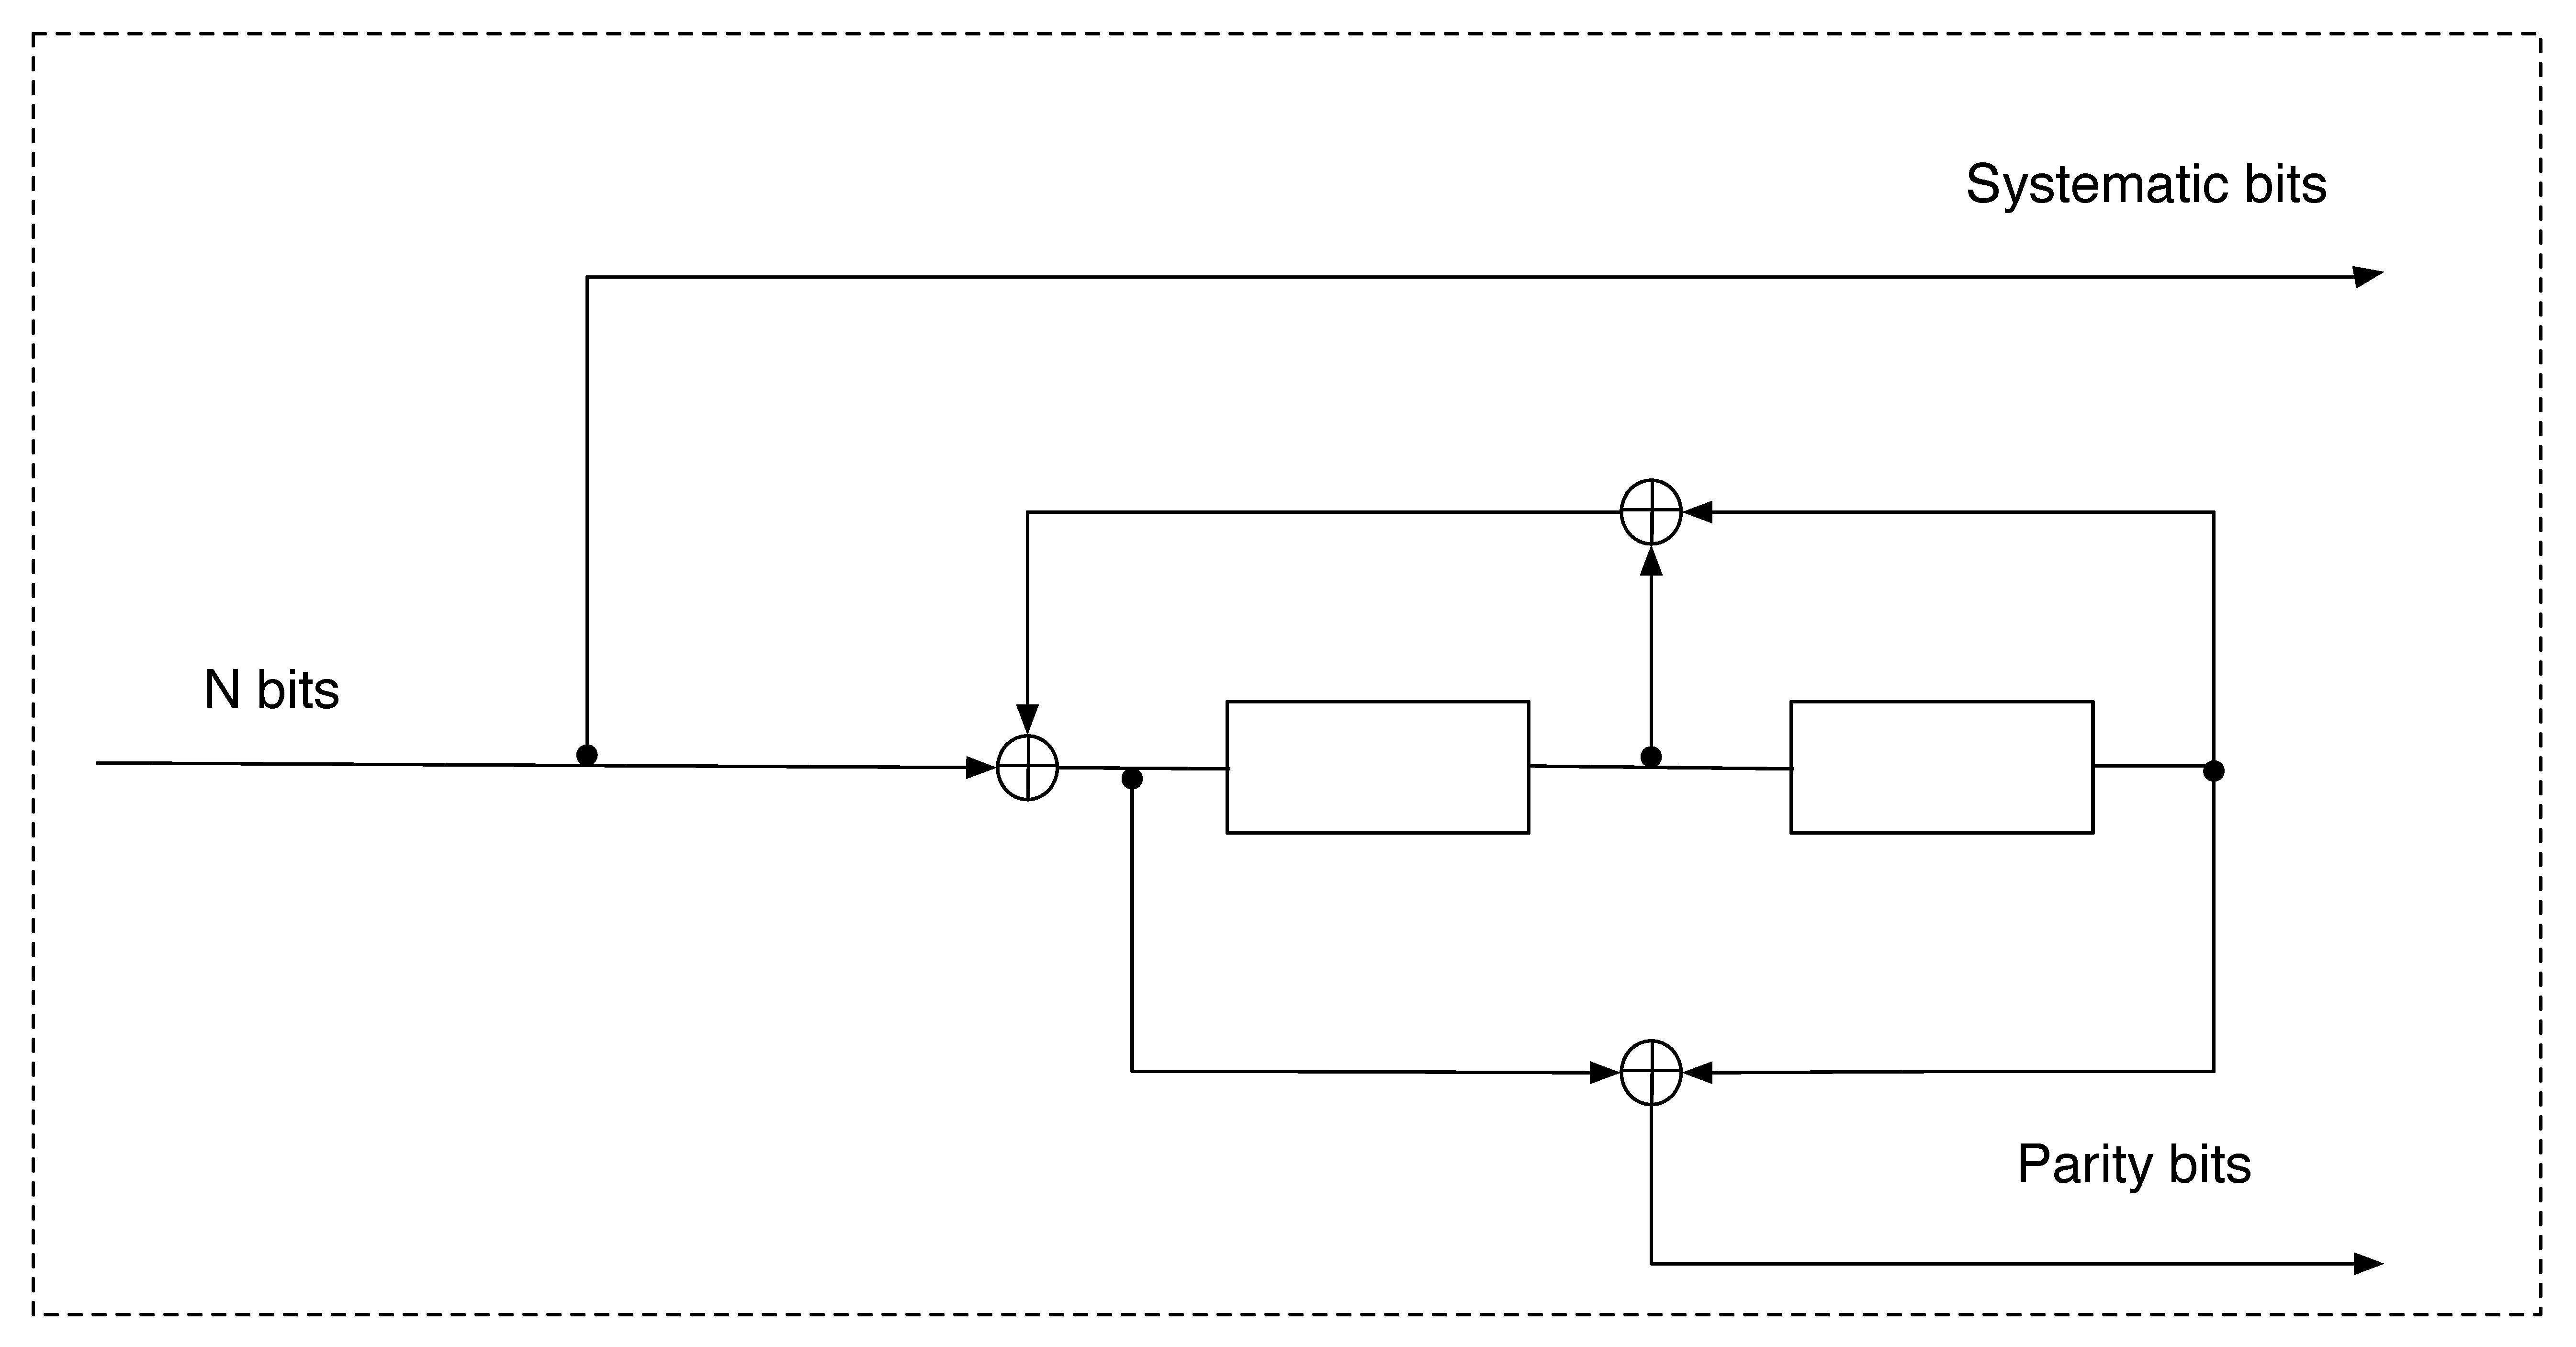
\includegraphics[width=0.45\textwidth]{./PaperSources/RSCExample3.pdf}
	%	\caption{$[\frac{1+x^2}{1+x+x^2}]$  RSC Encoder}
		%\label{fig1}
		%\end{figure}

%\begin{example}		
%An RSC encoder is shown in Figure \ref{fig1} with $k=1$ and $n=2$. Its parity generator\newline function is given by $[\frac{1+x^2}{1+x+x^2}]$, which may be written as $5/7$ in octal form, where $5 ~ \text{and} ~ 7$ correspond to the numerator and denominator of the generator function, respectively. 
 %For this RSC code, the cycle is $\bphi_g=\bphi_6 $ with a cycle length $\tau =3$. While $\bphi=(1~1~1~ 0~ 1~ 1~ 0~ 1~ 1~ 0~\cdots)$, which may be written in terms of the elements of GF(8) as $\bphi_7~\dot{\bphi_3}$ represents the impulse response. 
 %\end{example}
 % Moving forward all other examples and discussions relating to RSC codes will be done using the $5/7$ RSC code unless otherwise stated.

 %The knowledge of $\textbf{p}$ and $\tau$ will be used in deriving the method for determing which input messages generate low-weight parity bits. 
%\newpage
%\section{Distance Spectrum via Transfer Function of RSC Code}
\label{sec4}
The distance spectrum of an RSC code gives information about codeword weights and the number of codewords present in the code for a given weight generated as a result of message inputs that begin from, exit and then return to the zero state of the trellis of that code. Such message inputs are known as Return-to-Zero (RTZ) inputs. The distance spectrum of the RSC code can be obtained from its transfer function, denoted by $$T(Y,X)=\sum_{d=0}^{\infty}\sum_{w=0}^{\infty} a(d,w)Y^dX^w$$ where $a(d,w)$ is the number of codewords of weight $d$ generated by an input message of weight $w$.
Based on the method described in \cite{ref3}, we outline the process involved in deriving the transfer function of the $5/7$ RSC code. 

\begin{figure}[h]
\centering
		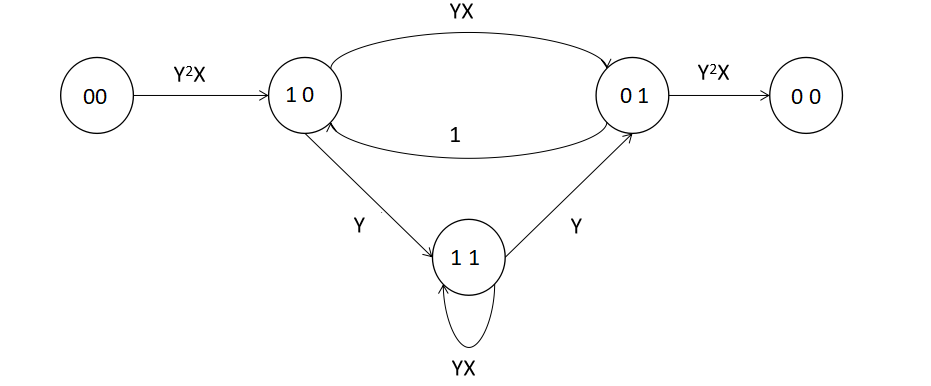
\includegraphics[width=0.45\textwidth]{tf.png}
		\caption{State Diagram of the $5/7$ RSC code }
		\label{Txfig4}
		\end{figure}
First, the state diagram of the $5/7$ RSC code is redrawn, as shown in Figure \ref{Txfig4}. The zero state is split into two and the transition from the zero state to itself is omitted. On each edge, the variables $Y^d$ and $X^w$ are used to represent the output weight $d$ and input weight $w$ of the path, respectively. We treat each edge label as a transfer block and employ the following rules for graph simplification:
Assume two edges labelled $H$ and $B$. Then,

\begin{enumerate}
\item If $H$ is connected in series to $B$, the labels are merged as $HB$.

\item If $H$ is connected in parallel to $B$, the labels are merged as $H+B$.

\item If the edges are in a feedback configuration, where $H$ and $B$ are the feedfoward and feedback portions respectively, the labels are merged as $\frac{H}{1-HB}$.
\end{enumerate}

In the following, we demonstrate the process for deriving the transfer function for the RSCC shown in Figure {\ref{Txfig4}}. The respective state diagram transformations are also shown in Figure {\ref{Txfig5}}.

\begin{figure}[h!]
\centering
		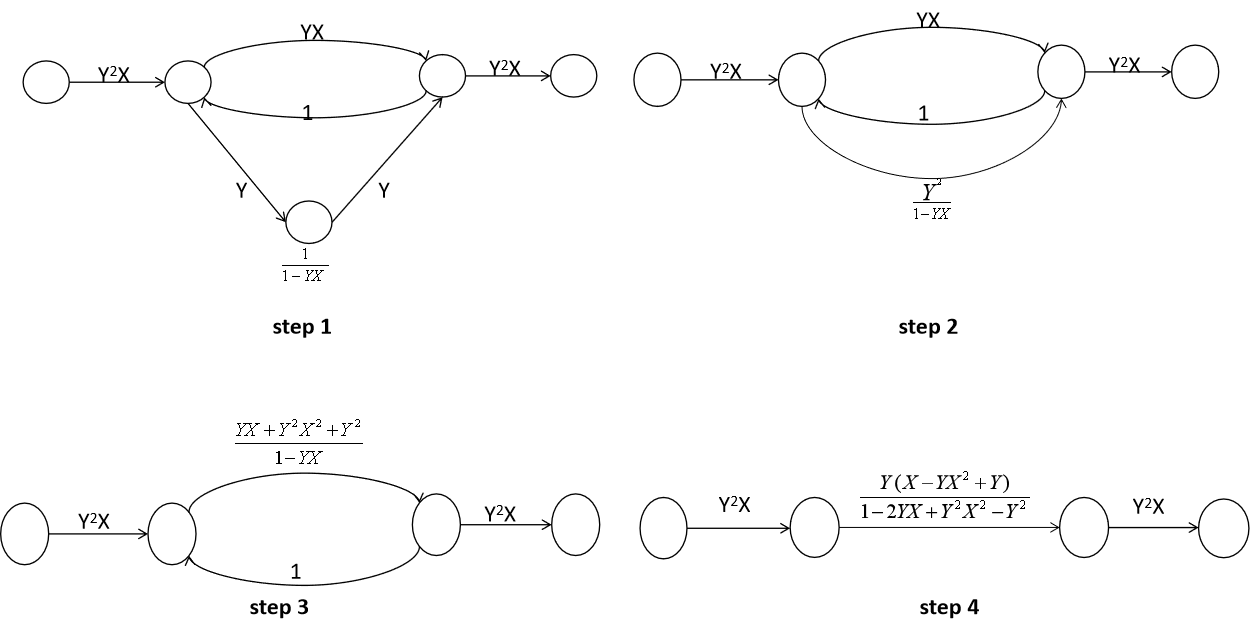
\includegraphics[width=0.5\textwidth]{tfexample.png}
		\caption{State Diagram Transformations involved in Transfer Function Calculation }
		\label{Txfig5}
		\end{figure}

\begin{example} Define all edge labels\\
\label{ex3}
 edge $ a\triangleq 0 0 \rightarrow 1 0$,  edge $b \triangleq 1 0 \rightarrow 0 1$\\
 edge $ c \triangleq 0 1 \rightarrow 0 0$, edge $d \triangleq 0 1 \rightarrow 1 0$\\
 edge $ e \triangleq 1 0 \rightarrow 1 1$, edge $f \triangleq 1 1 \rightarrow 1 1$\\
 edge $ g \triangleq 1 1 \rightarrow 1 0$

\begin{enumerate}
\item Simplify edge $g$ with feedback configuration

$$ \frac{1}{1-YX}$$

\item Merge edges $e,f,g$ with series configuration and rename it edge $h$

$$\text{edge}~h = Y\times \frac{1}{1-YX}\times Y=\frac{Y^2}{1-YX}$$

\item Merge edges $h,b$ with parallel configuration and rename it edge $j$

$$\text{edge}~j = YX+ \frac{Y^2}{1-YX}= \frac{YX+Y^2X^2+Y^2}{1-YX}$$

\item Merge  edges $j,d$ with feedback configuration and rename it edge $k$ 
\begin{equation*}
\begin{split}
 \text{edge}~k&= \frac{\frac{YX+Y^2X^2+Y^2}{1-YX}}{1-(\frac{YX+Y^2X^2+Y^2}{1-YX})}\\
 &=\frac{Y(X-YX^2+Y)}{1-2YX+Y^2X^2-Y^2}
\end{split}
\end{equation*}

\item Calculate transfer function by merging edges $k,a,c$ with series configuration

\begin{equation*}
\begin{split}
T(Y,X)&=Y^2X \times \frac{Y(X-YX^2+Y)}{1-2YX+Y^2X^2-Y^2}\times Y^2X \\
&=\frac{Y^5X^2(Y-YX^2+Y)}{1-2YX+Y^2X^2-Y^2}\\
&=Y^5X^3+Y^6(X^4+X^2)+Y^7(X^5+3X^3)+\\
&Y^8(X^6+6X^4+X^2)+Y^9(X^7+10X^5+5X^3)+...
\end{split}
\end{equation*}
\end{enumerate}
\end{example}

From the example, it is clear that the complexity involved in deriving the transfer function increases as the number of states of the RSCC increases and other methods such as Mason's Rule \cite{ref3} have to be used. Also to obtain the distance spectrum requires an extra division operation. In the case of interleaver design for Turbo codes, this method for generating the distance spectrum is not particularly useful. This is because it reveals no extra details with respect to the structure of the RTZ inputs. In the next section, we present a novel method whose complexity is independent of the number of states in the RSC code. As an added bonus, information regarding the structure of the RTZ inputs can be obtained using this method.
\section{Novel Method to Determine the Low-Weight Parity-Check Pattern}
\label{sec3}
In this section, we present our novel method for obtaining what we have named the \textit{codeword component pattern distance spectrum}. %Compared to the transfer function method, its complexity is independent of the number of states of the RSC. It is also able to reveal the pattern of low-weight codewords. 
Our novel method can be seen as the combination of two different but related methods. The first method is quite simple and makes use of the fact that in the polynomial domain, systematic components that are  RTZ inputs and their corresponding parity-check components share a common factor. 
The second method shows how to obtain this common factor when the weight of the parity check component is fixed for a given RSC code.  Through out this section, $c(x),~b(x)$ and $h(x)$ represesent the RSC codeword, the systematic component of the codeword and the parity check component of the codeword, respectively in polynomial notation.
%After explaining the inner working of our novel method, we used it to obtain the partial codeword pattern distance spectrum for the $5/7,~ 37/21$ and $23/35$  RSC codes.



\subsection{The Characteristics of Low-weight Codewords}
Since each RSC codeword is made up of two codeword components $b(x)$ and $h(x)$, it is obvious that the weight of the codeword $c(x)$ is given by 
\begin{equation}
w_H(c(x))=w_H(b(x)) + w_H(h(x))
\label{novelEq-1}
\end{equation} 
%(quarantine)%The distance spectrum derived via the transfer function method is an insufficient tool when it comes to to interleaver design. In this section, we present a novel method that generates what we refered to as the structured distance spectrum, which is the distance spectrum with the structure of the RTZ inputs as well as the corresponding parity-check sequence revealed, therefore making it a very useful tool for interleaver design.

%(quarantine)%For an RSC code, the Hamming weight of the codeword $w_H(\bc)$ is the sum of the weights of the parity bit sequence and message input. 
We first consider the parity check component, which can be expressed as 
\begin{equation}
h(x) =f(x)\cdot g^{-1}(x)\cdot b(x)
\label{novelEq0}
\end{equation}
If we consider large frame sizes, the presence of $g^{-1}(x)$ means that within $h(x)$ is a particular sequence of bits that is repeated a large number of times. This results in a large parity weight, and by extension, a relatively high-weight codeword. The only time this is not the case is when
\begin{equation}
b(x) \bmod g(x) \equiv 0
\label{novelEq1}
\end{equation}
This results in a relatively low-weight parity bit sequence, which might produce a low-weight codeword. Any $b(x)$ that meets the condition in (\ref{novelEq1}) can be written as 
\begin{equation}
b(x) =a(x)g(x)
\label{novelEq2}
\end{equation}
where $a(x)$ is a monic polynomial with $a_0=1$.
By fixing $b(x)$ from (\ref{novelEq2}) into (\ref{novelEq0}), we have 
\begin{equation}
\begin{split}
h(x)&=f(x)\cdot g^{-1}(x)\cdot a(x)g(x)\\
&=a(x)f(x)
\end{split}
\label{novelEq3}
\end{equation}
%(quarantine)%Using both (\ref{novelEq2})  and (\ref{novelEq3}), we wish to list all low-weight codewords for a given RSC code.A low-weight codeword is any codeword which satisfies the condition, $w_H(\bc) \leq d_{\text{max}}$. This list is known as the \textit{partial structured distance spectrum}. To generate the partial structured distance spectrum, we take note of a few things. 

%From (\ref{novelEq2})  and (\ref{novelEq3}), we observe that $a(x)$ is a common factor in both equations and if we are able to solve for $a(x)$ via either of the equations, the remaining equation can be solved. To solve for $a(x)$ requires that in either equation, it should be the only unknown variable. At first glance, it might seem that $g(x)$ and $f(x)$ are the only known variables because they are dependent on the RSC code in question. However, if we remember that the weight of $h(x)$ and $b(x)$ is directly proportional to the number of terms it has, then we are on our way to obtain our second known variable. What is left is to determine the valid power values for the polynomial  terms, depending on the weight of $h(x)$ or $b(x)$.

Thus, for a given $f(x)$ and $g(x)$, our goal is to find all $a(x)$s which generate low-weight codewords components in  (\ref{novelEq2}) and  (\ref{novelEq3}) simultaneously. 
However, since there is essentially no difference between the general structure of $h(x)$ and $b(x)$, we restrict our our attention to the low-weight parity check patterns in  (\ref{novelEq3}) and in the following, we present a method for determining valid values of $h(x)$ when $2 \leq w_H(h(x))\leq 3$. 
%In (\ref{novelEq3}), once $f(x)$ is given, our goal is to find $a(x)$ that results in a low-weight $h(x)$. To this end, we consider the roots of $f(x)$ 
%If $f(x)$ is a prime polynomial or can be factorized into prime polynomials, the the roots of $f(x)$ are its primitive elem
 %denoted by $\beta_i,~ 0 \leq i < 2^{m}-1)$. Then it is obvious that $h(\beta^i)=0$~ for all $\beta^i$ that are primitive elements 
%and we can reformulate our goal as to find weight-$w$ polynomials ($h(x)$) which take all the roots of $f(x)$ as its roots. The roots of $f(x)$ depend on its characteristic make-up and once that is known, we can easily determine the structure of $h(x)$ for a given value of $w_H(h(x))$. 
%The characteristic make-up of $f(x)$ can be grouped into the three cases below. 
%\begin{enumerate}
%\item Single primitive polynomial.
%\item Prime but not a primitive polynomial.
%\item Made up of repeated polynomial roots.
%\end{enumerate}


%It is worth noting that the method to be discussed can also be used to obtain valid values of $b(x)$, because there is no difference between the general structure of $h(x)$ and $b(x)$ once the Hamming weight is fixed. 
\subsection{The Characteristic of Weight $2$ Parity Check Pattern}
For this weight case, we can write $h(x)$ as $h(x)=1+x^a$ without any loss of generality. 
Let $M$ be the degree of $f(x)$ and $\alpha_m, ~0 \leq m \leq M-1$, be the roots of $f(x)$ satisfying $f(\alpha_m) = 0$ for all $0 \leq m \leq M-1$. Then from (\ref{novelEq3}), we have
\begin{equation}
\begin{split}
&h(\alpha_m)=0\\
&1+(\alpha_m)^a =0
\end{split}
\label{novelEq5b}
\end{equation}
for all $0 \leq m \leq M-1$ and therefore, we can reformulate our goal as to find low-weight polynomials $h(x)$ which satisfy (\ref{novelEq5b}) for all roots of $f(x)$. 

Now we consider the characteristics of the roots of $f(x)$ for the folowing 2 cases.
%Thus we wish to find the possible values of $a$ satisfying $$\beta^{ia}+1=0$$ for all $\beta^i,~1 \leq i \leq 2^{m}-1$ in GF$(2^{m}),~m=\text{order}(g(x))$
\paragraph{ Case1} $f(x)$ is a single irreducible polynomial\newline
For this case, $f(x)$ has $M$ distinct roots and each root $\alpha_m$ can be expressed as
\begin{equation}
\alpha_m=\beta^{2^m},~ 0\leq m \leq M-1
\end{equation}
where $\beta^{2^m}$ is primitive element in GF($2^M$) with order $\epsilon,~\epsilon | 2^M-1$. 
Now, if we consider the possible values of $a>0$ such that 
$$(\beta^{2^m})^a=1$$
then,
$$a \bmod \epsilon  \equiv 0$$
since $(\beta^{2^m})^{\epsilon}=1$

\begin{example}
$f(x)=1+x+x^2$.\newline $f(x)$ generates the field GF$(2^2)$. There are 2 distinct roots of $f(x)$, $\beta$ and $\beta^2$. The order of $\beta$ and $\beta^2$ is $\epsilon=3$, and the  valid values of $a$ are $a=\{3,6,9,\cdots \}$. The corresponding values for $a(x)$ and $h(x)$ are shown in Table \ref{novelTab2} for the first four valid values of $a$.
\begin{table}[htbp]
%\parbox{.5\linewidth}{
 \caption{$f(x)=1+x+x^2$}
\centering
 \begin{tabular}{c c c} 
%\hline
 $a(x)$ & $h(x)$ \\ [0.5ex] 
 \hline\hline
$1+x$
 & $1+x^{3}$ \\
\hline
$1+x+x^3+x^4$
 & $1+x^{6}$ 
 \\
\hline
$1+x+x^3+x^4+x^6+x^{7}$ 
&  $1+x^{9}$ 
\\
\hline
$1+x+x^3+x^4+x^6+x^{7}+x^9+x^{10}$
 &  $1+x^{12}$ \\
 \end{tabular}
 \label{novelTab2}
\end{table}
\end{example}
%============================
%\begin{example}$g(x)=1+x+x^4$\newline
%$g(x)$ can be used to generate the extended field GF$(2^4)$. In this field, $\beta^{15}=1$. The valid values of $a$ are $a=\{15,30,45,\cdots \}$. The corresponding values for $a(x)$ and $b(x)$ are shown in the table below for the first two valid values of $a$.
% \begin{table*}[h]
 %\caption{$23/35$ RSC Code, $f(x)=1+x+x^4$}
%\centering
%\begin{tabular}{p{4cm} | c} 
% \hline
 %$a(x)$ & $b(x)$  \\ [0.5ex] 
 %\hline\hline
%$1+x^2+x^3+x^5+x^7+x^8+x^{11}$ 
%& $1+x^{15}$ \\ 
%\hline
%$1+x^2+x^3+x^5+x^7+x^8+x^{11}+x^{15}+x^{16}+x^{17}+x^{18}+x^{20}+x^{22}+x^{23}+x^{26}$ 
%&$1+x^{30}$\\
 %\end{tabular}
 %\label{novelTab5}
%\end{table*}
%\end{example}
%=====================
%\paragraph{Case2}$f(x)$ is prime polynomial but not primitive \newline
%Similar to the case for primitive polynomials, we need to find the order of $\beta$. For fields generated by prime polynomials, there is a value $j < 2^m-1$ such that 
%$$\beta^j=1,~j~|~2^{m}-1 $$ where $j$ is the order. Therefore, any valid value of $a$ should satisfy the condition below.
%$$ a \bmod j \equiv 0$$

\begin{example}
$f(x)=1+x+x^2+x^3+x^4$\newline
$f(x)$ can be used used to generate GF$(2^4)$. There are 4 distinct roots and $\beta,~\beta^2,~\beta^3~\text{and}~\beta^4$. The order of each root is $\epsilon=5$ and therefore, the valid values of $a$ are $a=\{5,10,15,\cdots\}$. The corresponding values for $a(x)$ and $h(x)$ are shown in Table \ref{novelTab3} for the first four valid values of $a$.

%}
\begin{table}[htbp]
%\parbox{.5\linewidth}{
\caption{$f(x)=1+x+x^2+x^3+x^4$}
\centering
\begin{tabular}{c c} 
 \hline
 $a(x)$ & $h(x)$  \\ [0.5ex] 
 \hline\hline
$1+x$ &$1+x^5$\\ 
$1+x+x^5+x^6$ &$1+x^{10}$  \\
$1+x+x^5+x^6+x^{10}+x^{11}$ & $1+x^{15}$ \\
$1+x+x^5+x^6+x^{10}+x^{11}+x^{15}+x^{16}$ &$1+x^{20}$  
 \end{tabular}
 \label{novelTab3}
%}ll
\end{table}
\end{example}

%\paragraph{ Case3: $g(x)$ is made up of repeated polynomial roots.\newline}
%Given the above condition we have, $r(x)=(r^{o_p}_p(x))^k$, where $r^{o_p}_p(x)$ represents the prime polynomial $r(x)$ can be factorised into and $k$ is the number of times it is repeated. $r^{o_p}_p(x)$ has $\beta$ as its roots and we need to find $d \st \beta^j=1$ in the (extended) field it generates. Because $\beta^{kj}=1$ in the same (extended) field , the valid values for $a$ should satisfy the condition below:
%$$kj ~| ~a$$

\paragraph{Case2}$f(x)$ can be factorised into multiple irreducible polynomials. \newline
For this case, we can write $f(x)$ as $$f(x)=\prod_{k=1}^{K}f_k(x)$$ where $f_k(x)$ is an irreducible polynomial with order $\epsilon_k$. 
For each $f_k(x)$, the valid values of  $a_k$ are such that 
$$a_k \bmod \epsilon_k \equiv 0$$ and the valid values of $a$ are such that
$$a \in  \bigcap_{k=1}^{K} a_k$$
This means that $a$ satisfies the condition
$$ a \bmod  \prod_{k=1}^{K} \epsilon_k \equiv 0$$
For the special case where $f(x)$ can be factorised into equal irreducible polynomials, the above condition simplifies to 
$$a \bmod \epsilon K \equiv 0$$

\begin{example}
$f(x)=1+x^2$\newline
$f(x)$ can be written as $$f(x)=(1+x)^2,~K=2$$ $1+x$ is prime in $GF(2)$ and has $\beta$ as its root. The order of $\beta$ is $1$. Since $f(x)$ is made up of equal repeated polynomial and $K=2$, the valid values of $a=\{2,4,6,\cdots \}$.
The corresponding values for $a(x)$ and $h(x)$ are shown in Table \ref{novelTab1} for the first four valid values of $a$.
\begin{table}[htbp]
\renewcommand{\arraystretch}{1.3}
%\parbox{.3\linewidth}{
 \caption{$f(x)=1+x^2$}
 \centering
\begin{tabular}{c c } 
\hline
 $a(x)$ & $h(x)$ \\ [0.5ex] 
\hline\hline
$1$ & $1+x^2$\\ 
$1+x^2$ & $1+x^4$ \\
$1+x^2+x^4$ & $1+x^6$\\
$1+x^2+x^4+x^6$ & $1+x^8$ 
\end{tabular}
 \label{novelTab1}
\end{table}
\end{example}

%==========
%\begin{example}
%$g(x)=1+x^4$\newline $g(x)$ is made up of equal repeated polynomial roots and can be written as $$g(x)=(1+x)^4,~k=4$$. $1+x$ is prime in $GF(2)$ and $\beta^{1}=1$. Since $k=4$, we have $\beta^{k}=\beta^{4}=1$. $b(x)=1+x^b$ and the valid values of $a=\{4,8,12,\cdots \}$.
%The corresponding values for $a(x),~b(x)$ and $h(x)$ are shown in the table below for the first four valid values of $a$

%\begin{table*}[h]
%\caption{$g(x)=1+x^4$}
%\centering
 %\begin{tabular}{c c c} 
 %\hline
%$a(x)$ & $h(x)$ \\ [0.5ex] 
%\hline\hline
%$1$ &  $1+x^4$\\ 
%$1+x^4$ & $1+x^8$ \\
%$1+x^4+x^8$ & $1+x^{12}$ \\
%$1+x^4+x^8+x^{12}$ & $1+x^{16}$ 
%\end{tabular}
%\label{novelTab4}
%\end{table*}
%\end{example}

%========
%\begin{example}
%$g(x)=1+x^2+x^3+x^4$\newline
%$g(x)$ can be written as $$g(x)=(1+x)(1+x+x^3),~K=2$$
 %$1+x$ is prime in $GF(2^1)$ and $\beta^{1}=1$. $1+x+x^3$ is prime in $GF(2^3)$ and $\beta^{7}=1$. $b(x)=1+x^b$ and consequently, the valid values of $a$ that meet the condition $$ \bigcap_{k=1}^{K} \{j_k~| a\}$$ are $a=\{7,14,21,\cdots \}$.
%The corresponding values for $a(x)$ and $b(x)$ are shown in Table \ref{novelTab6} for the first four valid values of $a$
%\end{example}


%\hfill
%\parbox{\linewidth}{
%\begin{table*}[h]
%\caption{$g(x)=1+x^2+x^3+x^4$}
%\centering
% \begin{tabular}{p{4cm}| c} 
 %\hline
 %$a(x)$ & $b(x)$  \\ [0.5ex] 
 %\hline\hline
%$1+x^2+x^3$ & $1+x^7$ \\ 
%\hline
%$1+x^2+x^3+x^7+x^9+x^{10}$ &  $1+x^{14}$ \\
%\hline
%$1+x^2+x^3+x^7+x^{9}+x^{10}+x^{14}+x^{16}+x^{17}$ & $1+x^{21}$ 
%\\
%\hline
%$1+x^2+x^3+x^7+x^{9}+x^{10}+x^{14}+x^{16}+x^{17}+x^{21}+x^{23}+x^{24}$ & $1+x^{28}$
% \end{tabular}
 %\label{novelTab6}
%\end{table*}
%}
%\end{table}


\subsection{The Characteristic of Weight $3$ Parity Check Pattern}
For this weight case, 
\begin{equation}
h(x)=1+x^a+x^b,~a\neq b
\label{novelEqwt3}
\end{equation}
without loss of generality. We consider the characteristics of the roots of $f(x)$ for the folowing 2 cases.
%Given $f(x)$, our task is to find valid $(a,~b)$ pair values satisfying the condition 
%$$1+\beta^u+\beta^v=0$$
% If there are no values for the pair $(u,v)$, then $q(x) \st w_H(\bq) =3$ does not exist for the given $g(x)$.
% It is worth noting that such $h(x)$ only exist iff $f(x)$ has exactly $w_H(\bh) =3$ terms. Moving forward, we assume that for all the cases, this condition holds true.
\paragraph{ Case1} $f(x)$ is a single irreducible polynomial \newline
If $f(x)$ is an irreducible polynomial, then it can be used to generate the extended field GF($2^M$). The non-zero elements of the extended field are represented by $\beta^m,~1 \leq m \leq 2^M-1$. Also, from the discussion in the previous section, we know that $f(x)$ has $M$ distinct roots, one of them being $\beta$. Substituting $\beta$ into (\ref{novelEqwt3}), we get 
\begin{equation}
\begin{split}
&h(\beta)=0\\
&1+\beta^a+\beta^b=0
\end{split}
\label{novelEqwt3-1}
\end{equation}
We can then reformulate our task as to find all $\beta^m$ such that 
\begin{equation}
\beta^{\eta}+\beta^{\zeta}=1,~\eta \neq \zeta
\end{equation}
By refering to the table of the extended field for GF$(2^m)$, we can find the valid $(\eta,~\zeta)$ pairs $\st \beta^{\eta}+\beta^{\zeta}=1$. If there are no valid $(\eta,~\zeta)$ pairs, then there is no parity check component of weight $3$ for the given $f(x)$.
 We represent the set of $(\eta,~\zeta)$ pairs as 
$\bz=\{ (\eta_1,~\zeta_1) ,( \eta_2,~\zeta_2),\cdots\}$. Then, any valid value $(a,~b)$ values should satisfy the condition
\begin{equation}
(a,b) \equiv (\eta,~\zeta) \bmod \epsilon,~(\eta,~\zeta)\in \bz
\end{equation}
% since $\beta^{2^{m}-1}=1$.
\begin{example}
$f(x)=1+x+x^2$ \newline
The elements of GF$(2^2)$ are shown in Table \ref{novelTab7} and it is obvious that there is exactly 1 valid $(\eta,\zeta)$ pair $\st \beta^{\eta}+\beta^{\zeta} = 1$ and that is the pair $(1,2)$.
This means that valid values of the $(a,b)$ pairs are any values $\st (a,b) \equiv (1,2) \bmod 3$.  The corresponding values for $a(x)$ and $h(x)$ are shown in the table below for the first four valid values of $(a,b)$.
\end{example}

 \begin{table}[htbp]
 \caption{Non-zero Elements of GF$(2^2)$ generated by $f(x)=1+x+x^2$}
\centering
 \begin{tabular}{c c} 
 \hline
 power representation & actual value \\ [0.5ex] 
 \hline\hline
$\beta^0~=\beta^3=1$ & $1$\\
\hline
$\beta$ & $\beta$\\
\hline
$\beta^2$ &  $1+\beta$\\
\hline
 \end{tabular}
 \label{novelTab7}
\end{table}

\begin{table}[htbp]
 \caption{$f(x)=1+x+x^2$}
\centering
 \begin{tabular}{c c} 
 \hline
 $a(x)$ & $h(x)$\\ [0.5ex] 
 \hline\hline
$1$ & $1+x+x^2$\\ 
\hline
$1+x+x^2$ &  $1+x^2+x^4$\\
\hline
$1+x+x^3$ & $1+x^4+x^5$\\
\hline
$1+x^2+x^3$ & $1+x+x^5$ 
 \end{tabular}
 \label{novelTab8}
\end{table}

%\paragraph{Case2}$r(x)$ is prime but not a primitive polynomial\newline
%Similar to the case where $f(x)$ is primitive, we confirm the existence of $(e,f)$ pairs $ \st \beta^e + \beta^f =1$. If there are no values for the pair $(e,f)$, then there is no $h(x)$ such that $w_H(h(x)) =3$ for the given $f(x)$.
%We represent the set of $(e,f)$ pairs as 
%$\bz=\{ (e_1,f_1) , e_2,f_2),\cdots\} $. Then any valid value for $a$ and $b$ should satisfy the condition
%$$(a,b) \equiv (e,f) \bmod j,~(e,f)\in \bz$$ where $j$ is the order of $\beta$.

%\begin{example}
%$f(x)=1+x+x^2+x^3+x^4$ \newline
%From the table of the extended field generated by $f(x)$ (Table \ref{novelTab9}), we see that there are no valid $(e,~f)$ and as such $h(x) \st w_H(h(x))=3$ is non-existent for $f(x)=1+x+x^2+x^3+x^4$.


%\begin{table*}[h!]
% \parbox{\linewidth}{
%\caption{Non-zero Elements of GF$(2^4)$ generated by $f(x)=1+x+x^2+x^3+x^4$}
%\centering
 %\begin{tabular}{c c} 
 %\hline
 %power & polynomial \\ [0.5ex] 
% \hline\hline
%$\beta^0~=\beta^5=\beta^{10}=\beta^{15}=1$ & $1$\\
%\hline
%$\beta=\beta^6=\beta^{11}$ & $\beta$\\
%\hline
%$\beta^2=\beta^7=\beta^{12}$ &  $\beta^2$\\
%\hline
%$\beta^3=\beta^8=\beta^{13}$ &  $\beta^3$\\
%\hline
%$\beta^4=\beta^9=\beta^{14}$ &  $\beta^3+\beta^2+\beta+1$\\
 %\end{tabular}
% \label{novelTab9}
%}
%\end{table*}

%\end{example}

%\paragraph{Case3: $r(x)$ is made up of equal repeated polynomial roots\newline}
%For this case, we can write $r(x)$ as 
%$r(x)=(r^{o_p}_p(x))^k$, where $r^{o_p}_p(x)$ represents the prime polynomial, which is the root of $r(x)$ and $k$ is the number of times it is repeated. If $r^{o_p}_p(x)$ is a primitive polynomial and $m>1$, then from Case1 there are exactly $q=2^{(m-1)}-1~(e,~f)$ pairs $\st \beta^e+\beta^f=1,~e \neq f$ in set $\bz$. 
%If $r^{o_p}_p(x)$ is prime but not a primitive polynomial, then we determine the number of elements in the set $\bz$ directly from the table representing the field it generates.
% If we focus on $f^{o_p}_p(x)$ only, $(u',v')$ should satisfy the condition$$ (u',v') \equiv (e,f)\bmod 2^{m}-1,~(e, f) \in \bz$$. However, since $f(x)$ is made up of $f^{o_p}_p(x)$ repeated $k$ times, and $\beta^{ke}+\beta^{kf}=1$, the valid values for $u$ and $v$
 %should satisfy the condition
% $$(u,v)=(ku',kv'),~(u,v) \equiv (e,f)\bmod 2^{m}-1,~(e, f) \in \bz $$.

\paragraph{Case2}$f(x)$ can be factorised into multiple irreducible polynomials. \newline
We may write $f(x)$ as $$f(x)=\prod_{k=1}^{K}f_k(x)$$ where $f_k(x)$ is an irreducible polynomial with order $\epsilon_k$
For each $f_k(x)$, we refer to the table of the extended field it generates and form the set $\bz_k$, which contains all the valid $(\eta^{(k)},~\zeta^{(k)})$ pairs for that particular $f_k(x)$. If that set exists, then, for that $f_k(x)$ the following condition is met
\begin{equation}
(a_k,~b_k) \equiv (\eta^{(k)},~\zeta^{(k)}) \bmod \epsilon_k,~(\eta^{(k)},~\zeta^{(k)})\in \bz_k
\end{equation}
and 
\begin{equation}
(a,~b) \equiv \bigcup_{k=1}^{K} (\eta^{(k)},~\zeta^{(k)}) \bmod \epsilon_k,~(\eta^{(k)},~\zeta^{(k)})\in \bz_k
\end{equation}

For the special case where $f(x)$ can be factorised into equal irreducible polynomial, the above condition simplifies to 
 \begin{equation*}
 \begin{split}
 &(a,~b) \equiv (K\eta,~K\zeta) \bmod \epsilon,~(\eta,~\zeta) \in \bz \\
 \end{split}
 \end{equation*}
 
 \begin{example}
 $f(x)=1+x^2$ \newline $f(x)$ can be written as $(1+x)^2$. $(1+x)$ is a primitive polynomial for GF$(2)$. The elements in GF$(2)$ are $1$ and $\beta$. In this field,  there are no valid $(e,f)$ pair values; therefore, $h(x)$ such that  $w_H(h(x))=3$ does not exist for $f(x)=1+x^2$.
 \end{example}
 
  %\begin{example}
 %$g(x) = 1+x^4$.\newline
 %After factorisation, we have $g(x)=(1+x)^4. $(1+x) is a primitive polynomial that generates the field GF$(2)$ and in this field, there are also no valid $(e,~f)$ and as such $b(x) \st w_H(\bb)=3$ is also non-existent.
 %\end{example}
 
  %\begin{example}
 %$g(x)=1+x^2+x^3+x^4$.\newline
 % Upon factorising, we have $g(x)=(1+x)(1+x+x^3)$. Table \ref{novelTab12} shows the elements of GF$(2^3)$ generated by $(1+x+x^3)$ and we can confirm that there are three valid $(e,~f)$ pairs. However, since there are no valid $(e,~f)$ pairs in GF$(2)$, it also means that there cannot be any valid $(u,~v)$ pairs and $b(x) \st w_H(\bb)=3$ does not exist.
 
 %\begin{table*}[h]
 %\caption{Non-zero Elements of GF$(2^3)$ generated by $1+x+x^3$}
%\centering
 %\begin{tabular}{c c} 
 %\hline
 %power & polynomial \\ [0.5ex] 
 %\hline\hline
%$\beta^0~=\beta^{7}=1$ & $1$\\
%\hline
%$\beta$ & $\beta$\\
%\hline
%$\beta^2$ &  $\beta^2$\\
%\hline
%$\beta^3$ & $\beta+1$\\
%\hline
%$\beta^4$ &  $\beta^2+\beta$\\
%\hline
%$\beta^5$ & $\beta^2+\beta+1$\\
%\hline
%$\beta^6$ &  $\beta^2+1$\\
 %\end{tabular}
 %\label{novelTab12}
%\end{table*}
 %\end{example}

%\begin{example}
%$5/7$ RSC Code, $f(x)=1+x^2,~g(x)=1+x+x^2$\newline
%$f(x)$ is a match for Case3 and can be written as $(1+x)^2$. $(1+x)$ is a primitive polynomial for GF$(2)$. The elements in GF$(2)$ are $1$ and $\beta$. In this field,  there are no valid $(e,f)$; therefore, $h(x) \st w_H(\bh)=3$ does not exist.

%$g(x)$ is a match for Case1, i.e. it is a primitive polynomial for GF$(2^2)$ with $\beta^{3}=1$. 
%The elements of GF$(2^2)$ are shown in Table \ref{novelTab5} and it is obvious that there is exactly 1 ($q=2^{(2-1)}-1~=1$) valid $(e,f)$ pair $\st \beta^e+\beta^f = 1$ and that is $(1,2)$.
%This means that valid values of the $(u,v)$ pairs are any values $\st (u,v) \equiv (1,2) \bmod 3$.  The corresponding values for $a(x),~b(x)$ and $h(x)$ are shown in the table below for the first four valid values of $(u,v)$

% \begin{table*}[h]
 %\caption{Non-zero Elements of GF$(2^2)$ generated by $g(x)=1+x+x^2$}
%\centering
% \begin{tabular}{c c} 
% \hline
 %power representation & actual value \\ [0.5ex] 
% \hline\hline
%$\beta^0~=\beta^3=1$ & $1$\\
%\hline
%$\beta$ & $\beta$\\
%\hline
%$\beta^2$ &  $1+\beta$\\
% \end{tabular}
 %\label{novelTab7}
%\end{table*}

%\begin{table*}[h]
% \caption{$5/7$ RSC, $g(x)=1+x+x^2$}
%\centering
% \begin{tabular}{c c c} 
% \hline
% $a(x)$ & $b(x)$ & $h(x)$\\ [0.5ex] 
% \hline\hline
%$1$ & $1+x+x^2$ & $1+x^2$\\ 
%\hline
%$1+x+x^2$ &  $1+x^2+x^4$ & $1+x+x^3+x^4$ \\
%\hline
%$1+x+x^3$ & $1+x^4+x^5$ & $1+x+x^2+x^5$\\
%\hline
%$1+x^2+x^3$ & $1+x+x^5$  &$1+x^3+x^4+x^5$
 %\end{tabular}
 %\label{novelTab8}
%\end{table*}
%\end{example}

%\newpage

 
 %\begin{example}
%$37/21$ RSC Code, $f(x)=1+x+x^2+x^3+x^4,~g(x)=1+x^4$\newline
%$f(x)$ is a match for Case2, i.e. it is a prime but not a primitive polynomial. From the table of the extended field generated by $f(x)$ (Table \ref{novelTab9}), we see that there are no valid $(e,~f)$ and as such $h(x) \st w_H(\bh)=3$ is non-existent.


 %\begin{table*}[h]
 %\caption{Non-zero Elements of GF$(2^2)$ generated by $f(x)=1+x+x^2+x^3+x^4$}
%\centering
 %\begin{tabular}{c c} 
 %\hline 
 %power & polynomial \\ [0.5ex] 
 %\hline\hline
%$\beta^0~=\beta^5=\beta^{10}=\beta^{15}=1$ & $1$\\
%\hline
%$\beta=\beta^6=\beta^{11}$ & $\beta$\\
%\hline
%$\beta^2=\beta^7=\beta^{12}$ &  $\beta^2$\\
%\hline
%$\beta^3=\beta^8=\beta^{13}$ &  $\beta^3$\\
%\hline
%$\beta^4=\beta^9=\beta^{14}$ &  $\beta^3+\beta^2+\beta+1$\\
 %\end{tabular}
 %\label{novelTab9}
%\end{table*}

%$g(x)$ is a match for Case3, i.e. it is made up of equal repeated roots. After factorisation, we have $g(x)=(1+x)^4. $(1+x) is a primitive polynomial that generates the field GF$(2)$ and in this field, there are also no valid $(e,~f)$ and as such $b(x) \st w_H(\bb)=3$ is also non-existent.
%\end{example}
 
%\begin{example}
%$23/35$ RSC Code, $f(x)=1+x+x^4,~g(x)=1+x^2+x^3+x^4$ \newline
%$f(x)$ is a match for Case1, i.e. it is a primitive polynomial that can be used to generate the extended field GF$(2^4)$ with $\beta^{15}=1$.. The elements of GF$(2^4)$ are shown in Table \ref{novelTab10} and we can see that there are seven valid $(e,f)$ pairs.
 
 %This means that the valid values of the $(u,v)$ pairs are any values $\st (u,v) \equiv (e,f) \bmod 15, (e,f) \in \bz,~\bz=\{(1,4),~(2,8) ,~(3,14) ,~(5,10) ,~(6,13) ,~(7,9) ,~(11,12))$.
 %The corresponding values for $a(x),~b(x)$ and $h(x)$ are shown in Table \ref{novelTab11} below for the first four valid values of $(u,v)$
 
  %\begin{table*}[h]
 %\caption{Non-zero Elements of GF$(2^4)$ generated by $f(x)=1+x+x^4$}
%\centering
 %\begin{tabular}{c c} 
 %\hline
 %power & polynomial \\ [0.5ex] 
 %\hline\hline
%$\beta^0~=\beta^{15}=1$ & $1$\\
%\hline
%$\beta$ & $\beta$\\
%\hline
%$\beta^2$ &  $\beta^2$\\
%\hline
%$\beta^3$ & $\beta^3$\\
%\hline
%$\beta^4$ &  $\beta+1$\\
%\hline
%$\beta^5$ & $\beta^2+\beta$\\
%\hline
%$\beta^6$ &  $\beta^3+\beta^2$\\
%\hline
%$\beta^7$ & $\beta^3+\beta+1$\\
%\hline
%$\beta^8$ &  $\beta^2+1$\\
%\hline
%$\beta^9$ & $\beta^3+\beta$\\
%\hline
%$\beta^{10}$ &  $\beta^2+\beta+1$\\
%\hline
%$\beta^{11}$ & $\beta^3+\beta^2+\beta$\\
%\hline
%$\beta^{12}$ &  $\beta^3+\beta^2+\beta+1$\\
%\hline
%$\beta^{13}$ & $\beta^3+\beta^2+1$\\
%\hline
%$\beta^{14}$ &  $\beta^3+1$\\
% \end{tabular}
% \label{novelTab10}
%\end{table*}
 
% \begin{table*}[h]
% \caption{$23/35$ RSC, $f(x)=1+x+x^4$}
%\centering
% \begin{tabular}{c c c} 
% \hline
% $a(x)$ & $b(x)$ & $h(x)$\\ [0.5ex] 
% \hline\hline
%$1$ & $1+x^2+x^3+x^4$ & $1+x+x^4$\\ 
%\hline
%$1+x+x^2+x^3+x^5$ &  $1+x^2+x^3+x^4+x^8+x^9$ & $1+x^7+x^9$ \\
%\hline
%$1+x+x^2+x^3+x^5+x^7+x^8$ & $1+x^2+x^3+x^4+x^7+x^{12}$ & $1+x^{11}+x^{12}$\\
%\hline
%$1+x+x^4$ & $1+x+x^2+x^4+x^5+x^6+x^7+x^8$  &$1+x^2+x^8$
 %\end{tabular}
% \label{novelTab11}
%\end{table*}
 
% $g(x)$ is a match for Case4, i.e. it is made up of unique repeated roots. Upon factorising, we have $g(x)=(1+x)(1+x+x^3)$. Table \ref{novelTab12} shows the elements of GF$(2^3)$ generated by $(1+x+x^3)$ and we can confirm that there are three valid $(e,~f)$ pairs. However, since there are no valid $(e,~f)$ pairs in GF$(2)$, it also means that there cannot be any valid $(u,~v)$ pairs and $b(x) \st w_H(\bb)=3$ does not exist.
 
% \begin{table*}[h]
% \caption{Non-zero Elements of GF$(2^3)$ generated by $1+x+x^3$}
%\centering
 %\begin{tabular}{c c} 
% \hline
 %power & polynomial \\ [0.5ex] 
% \hline\hline
%$\beta^0~=\beta^{7}=1$ & $1$\\
%\hline
%$\beta$ & $\beta$\\
%\hline
%$\beta^2$ &  $\beta^2$\\
%\hline
%$\beta^3$ & $\beta+1$\\
%\hline
%$\beta^4$ &  $\beta^2+\beta$\\
%\hline
%$\beta^5$ & $\beta^2+\beta+1$\\
%\hline
%$\beta^6$ &  $\beta^2+1$\\
%\end{tabular}
% \label{novelTab12}
%\end{table*}
%\end{example}



%\subsubsection{Higher order weight:$w_H=4$}%: Equal Repeated Polynomial Roots}
%If $w_H(\bq)=4$, then $q(x) = 1+x^{u}+x^{v}+x^{w}$.
%Finding the structure of $q(x)$ when $w_H=4$ for general cases has proven to be a difficult problem, for which we have not found a feasible solution to. However, there is a special case where have been able to come up with a method for determining the structure of $q(x)$. 

%\paragraph{$r(x)=1+x^{2i},~i=1,2,...$}
%Since $q(x)$ is divisible by $r(x)$, the roots of $r(x)$ are also the roots of $q(x)$. Inserting $\beta$ into $q(x)$, we get

%$$1+\beta^{u}+\beta^{v}+\beta^{w} =0$$
%Taking the derivative of the above equation, we get 
%\begin{equation*}
%\begin{split}
% &u\beta^{u-1}+v\beta^{v-1}+w\beta^{w-1} =0 \\
% & u\beta^{u-1}+v\beta^{v-1}+w\beta^{w-1} \equiv 0 \bmod 2
% \end{split}
% \end{equation*}
%We can see that to satisfy the equation above, there are 2 possible cases
%\begin{enumerate}
%\item $(u,~v,~w)$ is made up of two odd numbers, one even number.
%\item $(u,~v,~w)$ are all even numbers.
%\end{enumerate}

%For a valid $(u,~v,~w)$, we fix it into $q(x)$ and if it is divisible by $q(x)$, then $(u,~v,~w)$ is valid.
%In summary, valid $(u,~v,~w)$ should satisfy the condition
%$$u+v+w \equiv 0\bmod 2, ~1+\beta^{u}+\beta^{v}+\beta^{w} \bmod r(x) \equiv 0$$

%\begin{example}
%$5/7$ RSC code $f(x)=1+x^2,~g(x)=1+x+x^2$\newline
%$f(x)$ satisfies the special condition case and we can use the method above to obtain valid values of $(u,~v,~,w)$. The corresponding values for $a(x),~b(x)$ and $h(x)$ are shown in Table \ref{novelTab16} for the first four valid values of $(u,~v,~,w)$.

% \begin{table*}[h]
% \caption{$5/7$ RSC, $f(x)=1+x^2,~w_H(\bh)=4$}
%\centering
 %\begin{tabular}{c c c} 
% \hline
% $a(x)$ & $b(x)$ & $h(x)$\\ [0.5ex] 
% \hline\hline
%$1+x$ & $1+x^3$ & $1+x+x^2+x^3$\\ 
%\hline
%$1+x+x^2$ &  $1+x^2+x^4$ & $1+x+x^3+x^4$ \\
%\hline
%$1+x+x^3$ & $1+x^4+x^5$ & $1+x+x^2+x^5$\\
%\hline
%$1+x^2+x^3$ & $1+x+x^5$  &$1+x^3+x^4+x^5$
% \end{tabular}
% \label{novelTab16}
%\end{table*}

%\end{example}
%\newpage
\section{Union Bound and the Codeword Component Pattern Distance Spectrum}
\label{sec4}
For a given RSC code, we have shown in the previous section that each codeword $c(x)$ is made up of $b(x)$ and $h(x)$ which have $a(x)$ as their common factor as shown in (\ref{novelEq2}) and (\ref{novelEq3}).
 Now, let $\cA_h(d)$ be the set of all $a(x)$ which yields weight-$d$ parity-check component \ie, $w_H(h(x))=w_H(a(x)f(x))=d$ for $a(x) \in \cA_h(d)$. 
Similarly $\cA_b(d)$ is the set of all $a(x)$ which yields weight-$d$ systematic component \ie, $w_H(b(x))=w_H(a(x)g(x))=d$ for $a(x) \in \cA_b(d)$
 and $\cA_c(d)$ is the set of all $a(x)$ which yields weight-$d$ codeword \ie, $w_H(c(x))=w_H(a(x)f(x))+ w_H(a(x)g(x))=d$ for $a(x) \in \cA_c(d)$.  

Then, the union bound of the bit-error rate can be calculated as \cite{ref4}
\begin{align}
P_b \leq \frac{1}{k} \sum_{d=d_{\text{free}}}^{\infty} \sum_{a(x) \in \cA_c(d)}w_H(a(x)g(x)) Q\Bigg( \sqrt{\frac{2dE_c}{N_0}}\Bigg)
\label{novelEq6-1}
\end{align}
However, since the high-weight codewords have minor contribution on the unioin bound, \eqref{novelEq6-1} can be further approximated by setting a limit on the maximum value of the codeword weight $d_{\text{max}}$, resulting in
\begin{align}
P_b \leq \frac{1}{k} \sum_{d=d_{\text{free}}}^{d_{\text{max}}} \sum_{a(x) \in \cA_c(d)}w_H(a(x)g(x)) Q\Bigg( \sqrt{\frac{2dE_c}{N_0}}\Bigg)
\label{novelEq7}
\end{align}
%In order to confirm the validity of our method, we use the values obtained from Tables \ref{novelTab8}, \ref{novelTab9} and \ref{novelTab10} to find the bounds for the BER of the RSC code, $P_b$.Finally, we compare the results obtained to $P_b$ found using the Transfer Function method as well as the simulation results.

On the other hand, since the weight of codeword is the summation of information and parity check parts as shown in (\ref{novelEq-1}), when $w_H(b(x)), w_H(h(x)) \geq 2$, we have
\begin{align}
\cA_c(d) = \bigcup_{\ell = 2}^{d-2} \left\{\cA_b(\ell) \cap \cA_h(d-\ell)\right\}
\label{Eq:exactset}
\end{align}
However, to determine $\cA_b(\ell)$ or $\cA_h(\ell)$ for a large $\ell$ is a complex task in general. Thus, in this paper, we replace the set $\cA_c(d)$ by the approximated set $\cA_c'(d)$ as defined in  (\ref{setApprox})
\begin{equation}
\begin{split}
\cA_c(d) \approx \cA_c'(d) &= \left\{\bigcup_{\ell = 2}^{\ell+\alpha} \left\{\cA_b(\ell) \cap \cA_h(d-\ell)\right\}\right\}\bigcup \\
&\left\{\bigcup_{\ell = 2}^{\ell+\alpha} \left\{\cA_b(d-\ell) \cap \cA_h(\ell)\right\}\right\}
\end{split}
\label{setApprox}
\end{equation}
where some codewords in $\cA_c(d)$ with $\ell \approx d-\ell$ may be ignored in $\cA_c'(d)$.

\begin{example}
 $\alpha=1$\newline
Let $d=7$. The $\cA_c'(7)$ becomes
\begin{equation*}
\begin{split}
\cA_c'(7) &= \left\{\left\{\cA_b(2) \cap \cA_h(7-2)\right\} \bigcup  \left\{\cA_b(3) \cap \cA_h(7-3)\right\} \right\} \bigcup \\
& \left\{\left\{\cA_b(7-2) \cap \cA_h(2)\right\} \bigcup  \left\{\cA_b(7-3) \cap \cA_h(3)\right\} \right\} \\
&=\left\{\left\{\cA_b(2) \cap \cA_h(5)\right\} \bigcup  \left\{\cA_b(3) \cap \cA_h(4)\right\} \right\} \bigcup \\
& \left\{\left\{\cA_b(5) \cap \cA_h(2)\right\} \bigcup  \left\{\cA_b(4) \cap \cA_h(3)\right\} \right\} \\
\end{split}
\end{equation*}

If we set $d=8$, $\cA_c'(8)$ becomes
\begin{equation*}
\begin{split}
\cA_c'(8) &= \left\{\left\{\cA_b(2) \cap \cA_h(8-2)\right\} \bigcup  \left\{\cA_b(3) \cap \cA_h(8-3)\right\} \right\} \bigcup \\
& \left\{\left\{\cA_b(8-2) \cap \cA_h(2)\right\} \bigcup  \left\{\cA_b(8-3) \cap \cA_h(3)\right\} \right\} \\
&=\left\{\left\{\cA_b(2) \cap \cA_h(6)\right\} \bigcup  \left\{\cA_b(3) \cap \cA_h(5)\right\} \right\} \bigcup \\
& \left\{\left\{\cA_b(6) \cap \cA_h(2)\right\} \bigcup  \left\{\cA_b(5) \cap \cA_h(3)\right\} \right\} \\
\end{split}
\end{equation*}

We can see that $\left\{\cA_b(4) \cap \cA_h(4)\right\}$ is not used in $\cA_c'(8)$, event though it is used in $\cA_c(8)$.
\end{example}





%Having determined how to find valid values of $b(x)$ and $h(x)$ for Hamming weights $\leq 3$, we are now in a position to generate the codeword pattern distance spectrum for a given RSC code. We take a union bound like approach towards the generation of the codeword pattern distance spectrum. The approach is outlined below.
%\begin{enumerate}
 %\item Beginning with (\ref{novelEq2}), we find all values of $b(x),~w_H(b(x))=2$ that have the same roots as $g(x)$ and divide $g(x)$ by each valid polynomial to obtain the corresponding $a(x)$.\label{ubStep1}
 %\item Then using (\ref{novelEq3}), we multiply each $a(x)$ by $f(x)$ to obtain the corresponding value of $h(x)$. It is worth noting that $w_H(h(x))$ may be $\geq w_H(b(x))$. \label{ubStep2}
 %\item Since we are interested in only the low weight codewords, we ignore any $b(x) \st w_H(b(x))+w_H(h(x)) \geq d_{\text{max}}$. \label{ubStep3}
 %\item Next we set the weight value of $b(x)$ to $w_H(b(x))=3$, and repeat steps \ref{ubStep1} and \ref{ubStep2} while ignoring $b(x)$ that meet the condition in step \ref{ubStep3}.\label{ubStep4}
 %\item To obtain a complete codeword pattern distance spectrum, we do a reverse operation, \textit{i.e.} we focus on (\ref{novelEq2}) and find all values of $g(x),~w_H(\bh)=2$ that have the same roots as $f(x)$ and divide $f(x)$ by each valid polynomial to obtain the corresponding $a(x)$.
 %\item Then using (\ref{novelEq2}), we repeat steps \ref{ubStep2} through \ref{ubStep4}, being careful to avoid repitition.
 %\item Finally we arrange all valid values of $b(x)$ and $h(x)$ in ascending value of codeword weight,$w_H(b(x)) + w_H(h(x))$.
 %\end{enumerate}

%We use the codeword pattern distance spectrum to calculate the bit-error bounds for each RSC and compare them to the bit-error bounds obtained via the distance spectrum as well as simulation results. We use the probability of bit-error in doing this and a more general formula for calculating $P_b$ is shown below [4]:

%\begin{equation}
%P_b \leq \frac{1}{k} \sum_{d=d_{\text{free}}}^{\infty} w(d) Q\Bigg( \sqrt{\frac{2dE_c}{N_0}}\Bigg)
%\label{novelEq6}
%\end{equation}
%where $w(d)=\sum_{i=1}^{\infty} i~ a(d,i)$ and $ a(d,i)$ is the number of codewords of weight $d$ generated by an input message of weight $i$. If we set a limit on the maximum value of the codeword weight $d_{\text{max}}$
% we can rewrite (\ref{novelEq6}) as 
%\begin{equation}
%P_b \leq \frac{1}{k} \sum_{d=d_{\text{free}}}^{d_{\text{max}}} w(d) Q\Bigg( \sqrt{\frac{2dE_c}{N_0}}\Bigg)
%\label{novelEq7}
%\end{equation}
 %From the simulation results, we observed $d_{\text{max}}=d_{\text{min}}+3$ is a sufficient value for obtaining the BER bounds.
%In order to confirm the validity of our method, we use the values obtained from Tables \ref{novelTab8}, \ref{novelTab9} and \ref{novelTab10} to find the bounds for the BER of the RSC code, $P_b$.Finally, we compare the results obtained to $P_b$ found using the Transfer Function method as well as the simulation results.







%\newpage
\section{Results}
\label{sec5}
In this section, we compare the bounds obtained via our novel method to bounds obtained using the transfer function method as well as the simulation results for three different RSC codes, each with a frame size $N=64$. 
%For each RSC code and a frame size of $N=64$, the codeword is BPSK modulated and transmitted over the AWGN channel. At the receiver end, the Viterbi algorithm is used to decode before a decision is made on the decoded sequence.

The partial codeword component pattern distance spectrum for the $5/7,~37/21$ and $23/35$ RSC codes are shown in Tables \ref{novelTab13},  \ref{novelTab14} and \ref{novelTab15} respectively. 
%It is worth noting that in all the tables, the codeword components are arranged in ascending order of codeword weight, with the $d_{\text{free}}$ components at the top of the table.  
From the simulation results, we observed $d_{\text{max}}=d_{\text{min}}+3$ is a sufficient value for obtaining the BER bounds.
%(quarantine)%For each RSC codeThese were obtained by dividing the general form of $h(x)$ for $w_H(\bh)=2$ and ($w_H(\bh)=2$ if it exists) by $f(x)$ and multiplying it by $g(x)$ to obtain $b(x)$ for a given RSC code. This process is repeated doing the same for the general form of $b(x)$. In both cases $a(x),~b(x)$ and $h(x)$ are only added to the list if $w_H(\bc) \leq d_{\text{max}}$.

\begin{table}[htbp]
 \caption{Partial Codeword Component Pattern Distance Spectrum for the $5/7$ RSC code, $d_{\text{max}}=8$}
\centering
 \begin{tabular}{c c c} 
 \hline
 $a(x)$ & $b(x)$ & $h(x)$ \\ [0.5ex] 
 \hline\hline
$1$ & $1+x+x^{2}$ & $1+x^2$\\
\hline
$1+x^2$ & $1+x+x^3+x^4$ & $1+x^{4}$\\
\hline
$1+x$ & $1+x^3$ & $1+x+x^2+x^3$\\
\hline
$1+x^2+x^4$ & $1+x+x^3+x^5+x^6$ & $1+x^{6}$\\
\hline
$1+x^2+x^3$ & $1+x+x^5$ & $1+x^3+x^4+x^5$\\
\hline
$1+x+x^2$ & $1+x^2+x^4$ & $1+x+x^3+x^4$\\
\hline
$1+x+x^3$ & $1+x^4+x^5$ & $1+x+x^2+x^5$\\
\hline
$1+x^2+x^4+x^6$ & $1+x+x^3+x^5+x^7+x^8$ & $1+x^8$\\
\hline
$1+x+x^3+x^4$ & $1+x^6$ & $1+x+x^2+x^4+x^5+x^6$\\
%======extra
%\hline
%$1+x+x^3+x^5$ & $1+x^4+x^6+x^7$ & $1+x+x^2+x^7$\\
%\hline
%$1+x+x^2+x^4$ & $1+x^2+x^5+x^6$ & $1+x+x^3+x^6$\\
%\hline
%$1+x+x^2+x^3$ & $1+x^2+x^3+x^5$ & $1+x+x^4+x^5$\\
%\hline
%$1+x^2+x^3+x^5$ & $1+x+x^6+x^7$ & $1+x^3+x^4+x^7$\\
%\hline
%$1+x^2+x^3+x^4$ & $1+x+x^4+x^6$ & $1+x^3+x^5+x^6$\\
%\hline
%$1+x^2+x^4+x^5$ & $1+x+x^3+x^7$ & $1+x^5+x^6+x^7$\\
 \end{tabular}
 
 \label{novelTab13}
\end{table}

\begin{table}[h!]
 \caption{Partial Codeword Component Pattern Distance Spectrum for the $37/21$ RSC code,$d_{\text{max}}=9$}
\centering
 \begin{tabular}{c c c} 
 \hline
 $a(x)$ & $b(x)$ & $h(x)$ \\ [0.5ex] 
 \hline\hline
$1+x$ & $1+x+x^{4}+x^5$ & $1+x^5$\\
\hline
$1$ & $1+x^4$ & $1+x+x^2+x^3+x^4$\\
\hline
$1+x+x^5+x^6$ & $1+x+x^4+x^6+x^9+x^{10}$ & $1+x^{10}$\\
%\hline
%$1+x+x^4+x^5$ & $1+x+x^8+x^9$ & $1+x^4+x^5+x^9$\\
%\hline
%$1+x^2$ & $1+x^2+x^4+x^6$ & $1+x+x^5+x^6$\\
%\hline
%$1+x+x^5$ & $1+x+x^4+x^9$ & $1+x^6+x^7+x^8+x^9$\\
%\hline
%$1+x+x^4$ & $1+x+x^5+x^8$ & $1+x^4+x^6+x^7+x^8$\\
%\hline
%$1+x^2+x^4$ & $1+x^2+x^6+x^8$ & $1+x+x^4+x^7+x^8$\\
%\hline
%$1+x^3+x^4$& $1+x^3+x^7+x^8$ & $1+x+x^2+x^4+x^8$\\
%\hline
%$1+x^4+x^5$ & $1+x^5+x^8+x^9$ & $1+x+x^2+x^3+x^9$\\
 \end{tabular}
 
 \label{novelTab14}
\end{table}

\begin{table}[h!]
 \caption{Partial Codeword Component Pattern Distance Spectrum for the $23/35$ RSC code,$d_{\text{max}}=10$}
\centering
 \begin{tabular}{c c c} 
 \hline
 $a(x)$ & $b(x)$ & $h(x)$ \\ [0.5ex] 
 \hline\hline
$1+x^2+x^3$ & $1+x^7$ & $1+x+x^2+x^6+x^7$\\
\hline
$1$ & $1+x^2+x^3+x^4$ & $1+x+x^{4}$\\
\hline
$1+x+x^2+x^3+x^5$ & $1+x^3+x^4+x^8+x^9$ & $1+x^7+x^9$\\
\hline
$1+x+x^2+x^3+x^5+x^7+x^8$ & $1+x+x^3+x^4+x^7+x^{12}$ & $1+x^{11}+x^{12}$\\
\hline
$1+x^2+x^3+x^7+x^9+x^{10}$ & $1+x^{14}$ & $1+x+x^2+x^6+x^8+x^9+x^{13}+x^{14}$\\
 \end{tabular}
 
 \label{novelTab15}
\end{table}

\begin{figure}[h!]
\centering
		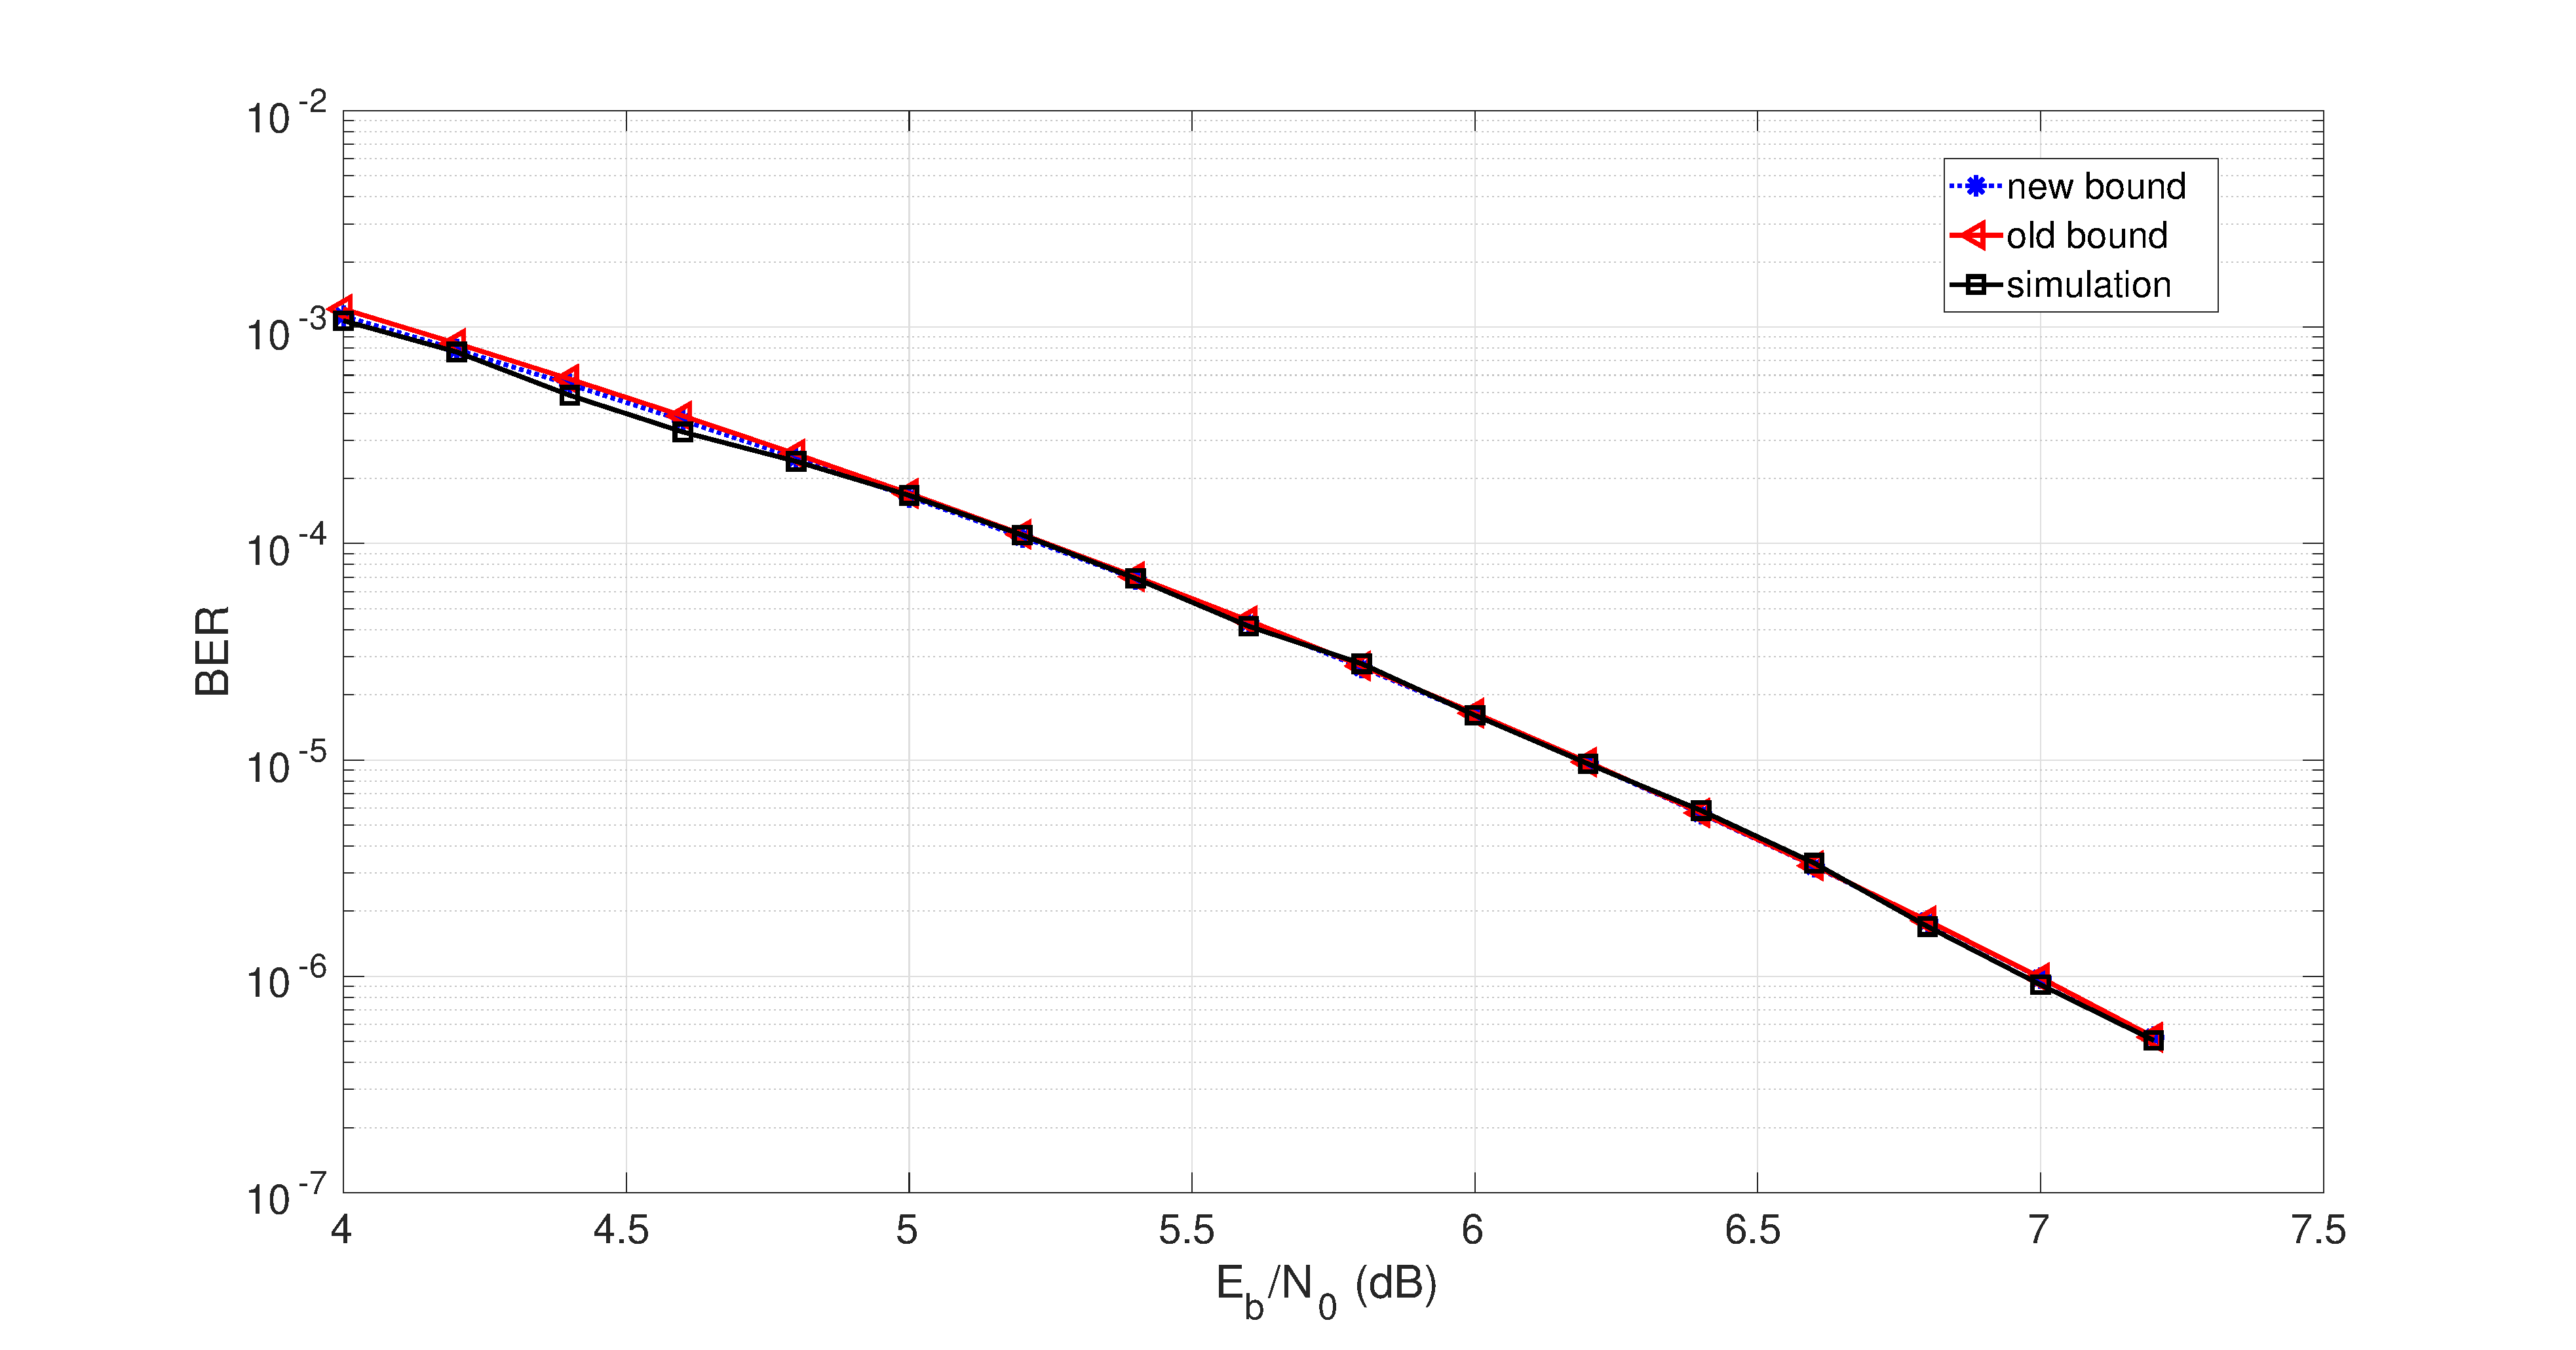
\includegraphics[width=0.5\textwidth]{./Images/RSC_5_7_lower_weights.eps}
		\captionof{figure}{Old Bound vs New Bound vs Simulation for 5/7 RSC Code}
		\label{simFig1}
		\end{figure}
		
%Fig. \ref{simFig1} shows the simulation results for the $5/7$ RSC code as well as the lower bounds obtained using the transfer function as well as our novel method. The feedforward connection has the polynomial representation $1+x^2$ and can be factorized into 2 irreducible polynomials, which means there are no low-weight codewords with parity-check components of weight $3$. The feedback connection has the polynomial representation $1+x+x^2$, which is an irreducuble polynomial and the order $\epsilon = 3$. This means that the low-weight codewords have systematic components with weight $2$ and weight $3$. In Fig. \ref{simFig1}, we observe that there is some difference between the new (novel method) bound and the old (transfer function) bound, but they tend to converge as $E_b/N_0$ increases. This suggests that the approximation used in our novel method is sufficient for this RSC code.

We observe that for both Fig. \ref{simFig1} and Fig. \ref{simFig2}, there is some difference between the new (novel method) bound and the old (transfer function) bound, but they tend to converge as $E_b/N_0$ increases. This suggests that the approximation used with our novel method is sufficient for these RSC codes.

%codewords generated considering $b(x),~w_H(b(x))>3$ as well as codewords which have a parity-check sequence $h(x),~w_H(h(x))>3$ do not have much effect on the BER of the code as $E_b/N_0$ increases.

%The gap that is observed in the low $E_b/N_0$ regions is attributed to omitting codewords generated by the RTZ inputs of weight $w_H(\bb)=4$ as well as codewords with parity-check sequences $w_H(\bh)=4$ in our calculation of the new bound. 

%Fig. \ref{simFig4} and Fig. \ref{simFig5} are similar to  Fig. \ref{simFig1} and Fig. \ref{simFig2}, with the only difference being that codewords generated by the RTZ inputs of weight $w_H(\bb)=4$ as well as codewords with parity-check sequences $w_H(\bh)=4$ have been added in our calculation of the new bound. The new and old bounds match up and the accuracy of our bound is greatly improved.The simulation results also agree with the bounds as they also converge with the bounds.

\begin{figure}[h!]
\centering
		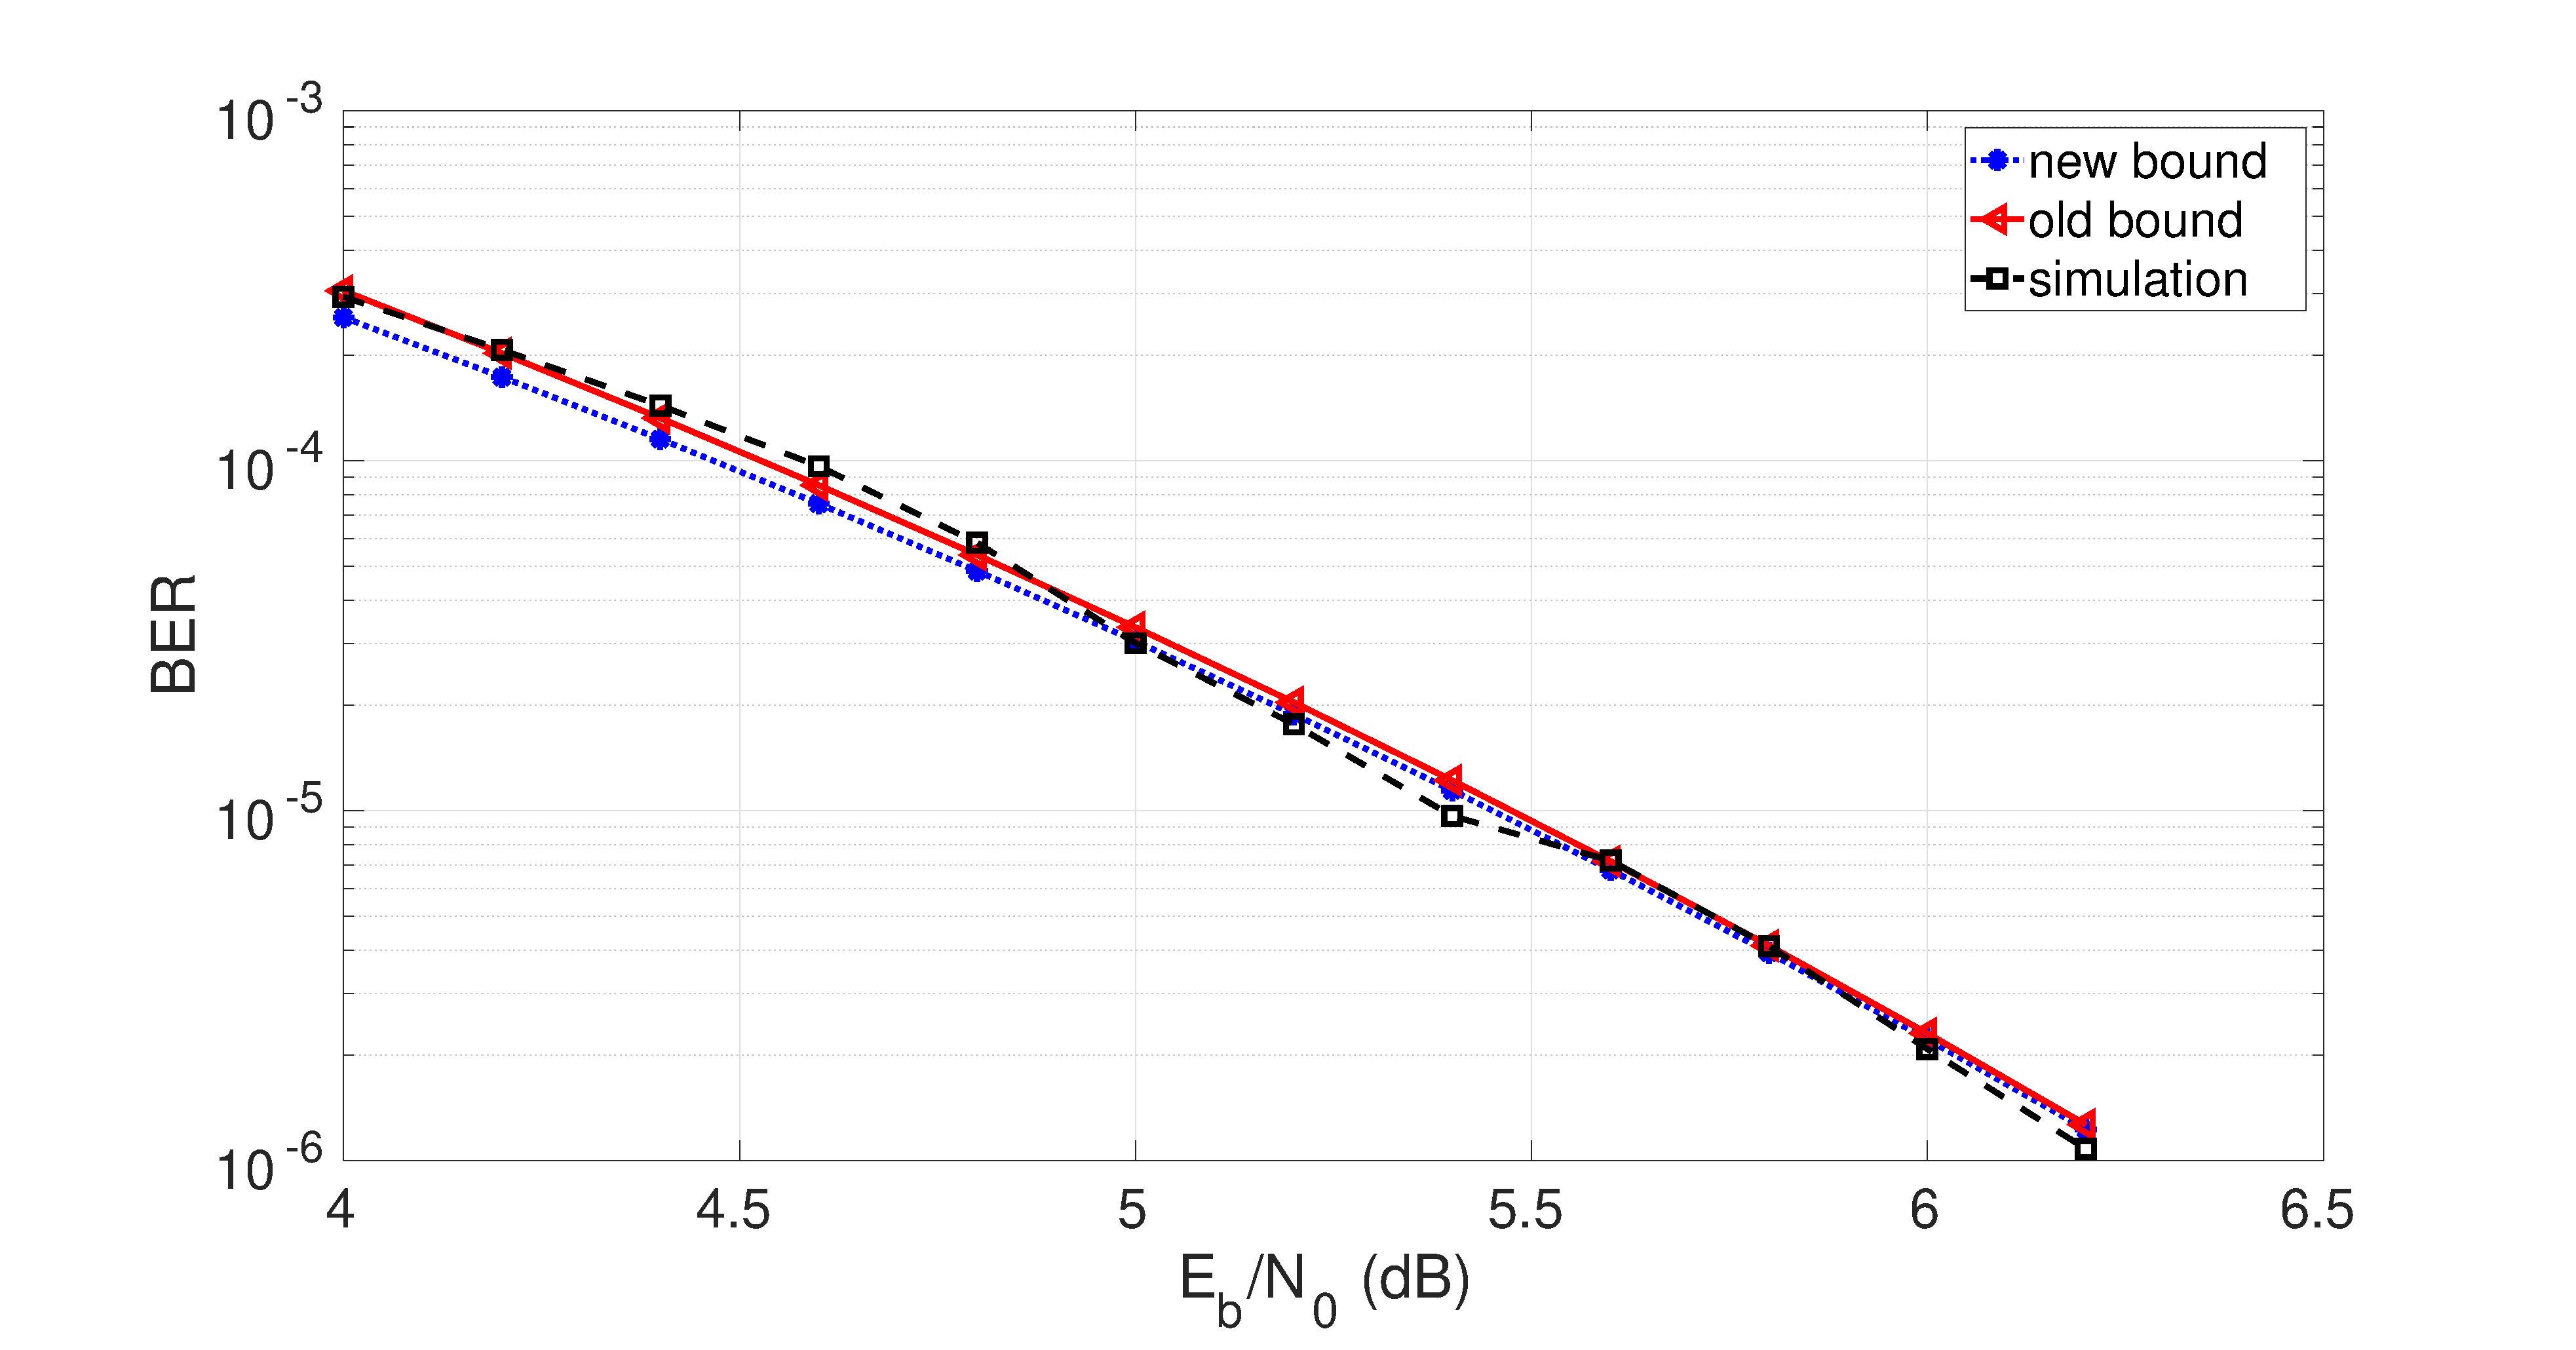
\includegraphics[width=0.5\textwidth]{./Images/RSC_37_21_lower_weights.eps}
		\caption{Old Bound vs New Bound vs Simulation for 37/21 RSC Code}
		\label{simFig2}
		\end{figure}
%Fig. \ref{simFig2} shows the simulation results for the $37/21$ RSC code as well as the lower bounds obtained using the transfer function as well as our novel method. The feedforward connection has the polynomial representation $1+x+x^2+x^3+x^4$, which is an irreducible polynomial. However, we observe from Table \ref{novelTab14} that the codeword has no parity check components of weight $3$. The feedback connection has the polynomial representation $1+x^4$, which can be factorized into $4$ and there are no low-codewords with systematic components of weight $3$. In Fig. \ref{simFig2}, we observe that there is some difference between the new (novel method) bound and the old (transfer function) bound, but they tend to converge as $E_b/N_0$ increases. Again, this suggests that the approximation used in our novel method is sufficient for this RSC code.
In \ref{simFig3}, we observe that the old bounds and simulation results converge as the Eb/No value increases. However, there is a very distinct gap between the new bound and the old bound. Moreover, the bounds do not converge as the Eb/No increases. This suggests that the approximation used in our novel method is insufficient for this RSC code and considering  $w_H(h(x)),~w_H(b(x))=4$ might yield a more accurate bound.

\begin{figure}[h!]
\centering
		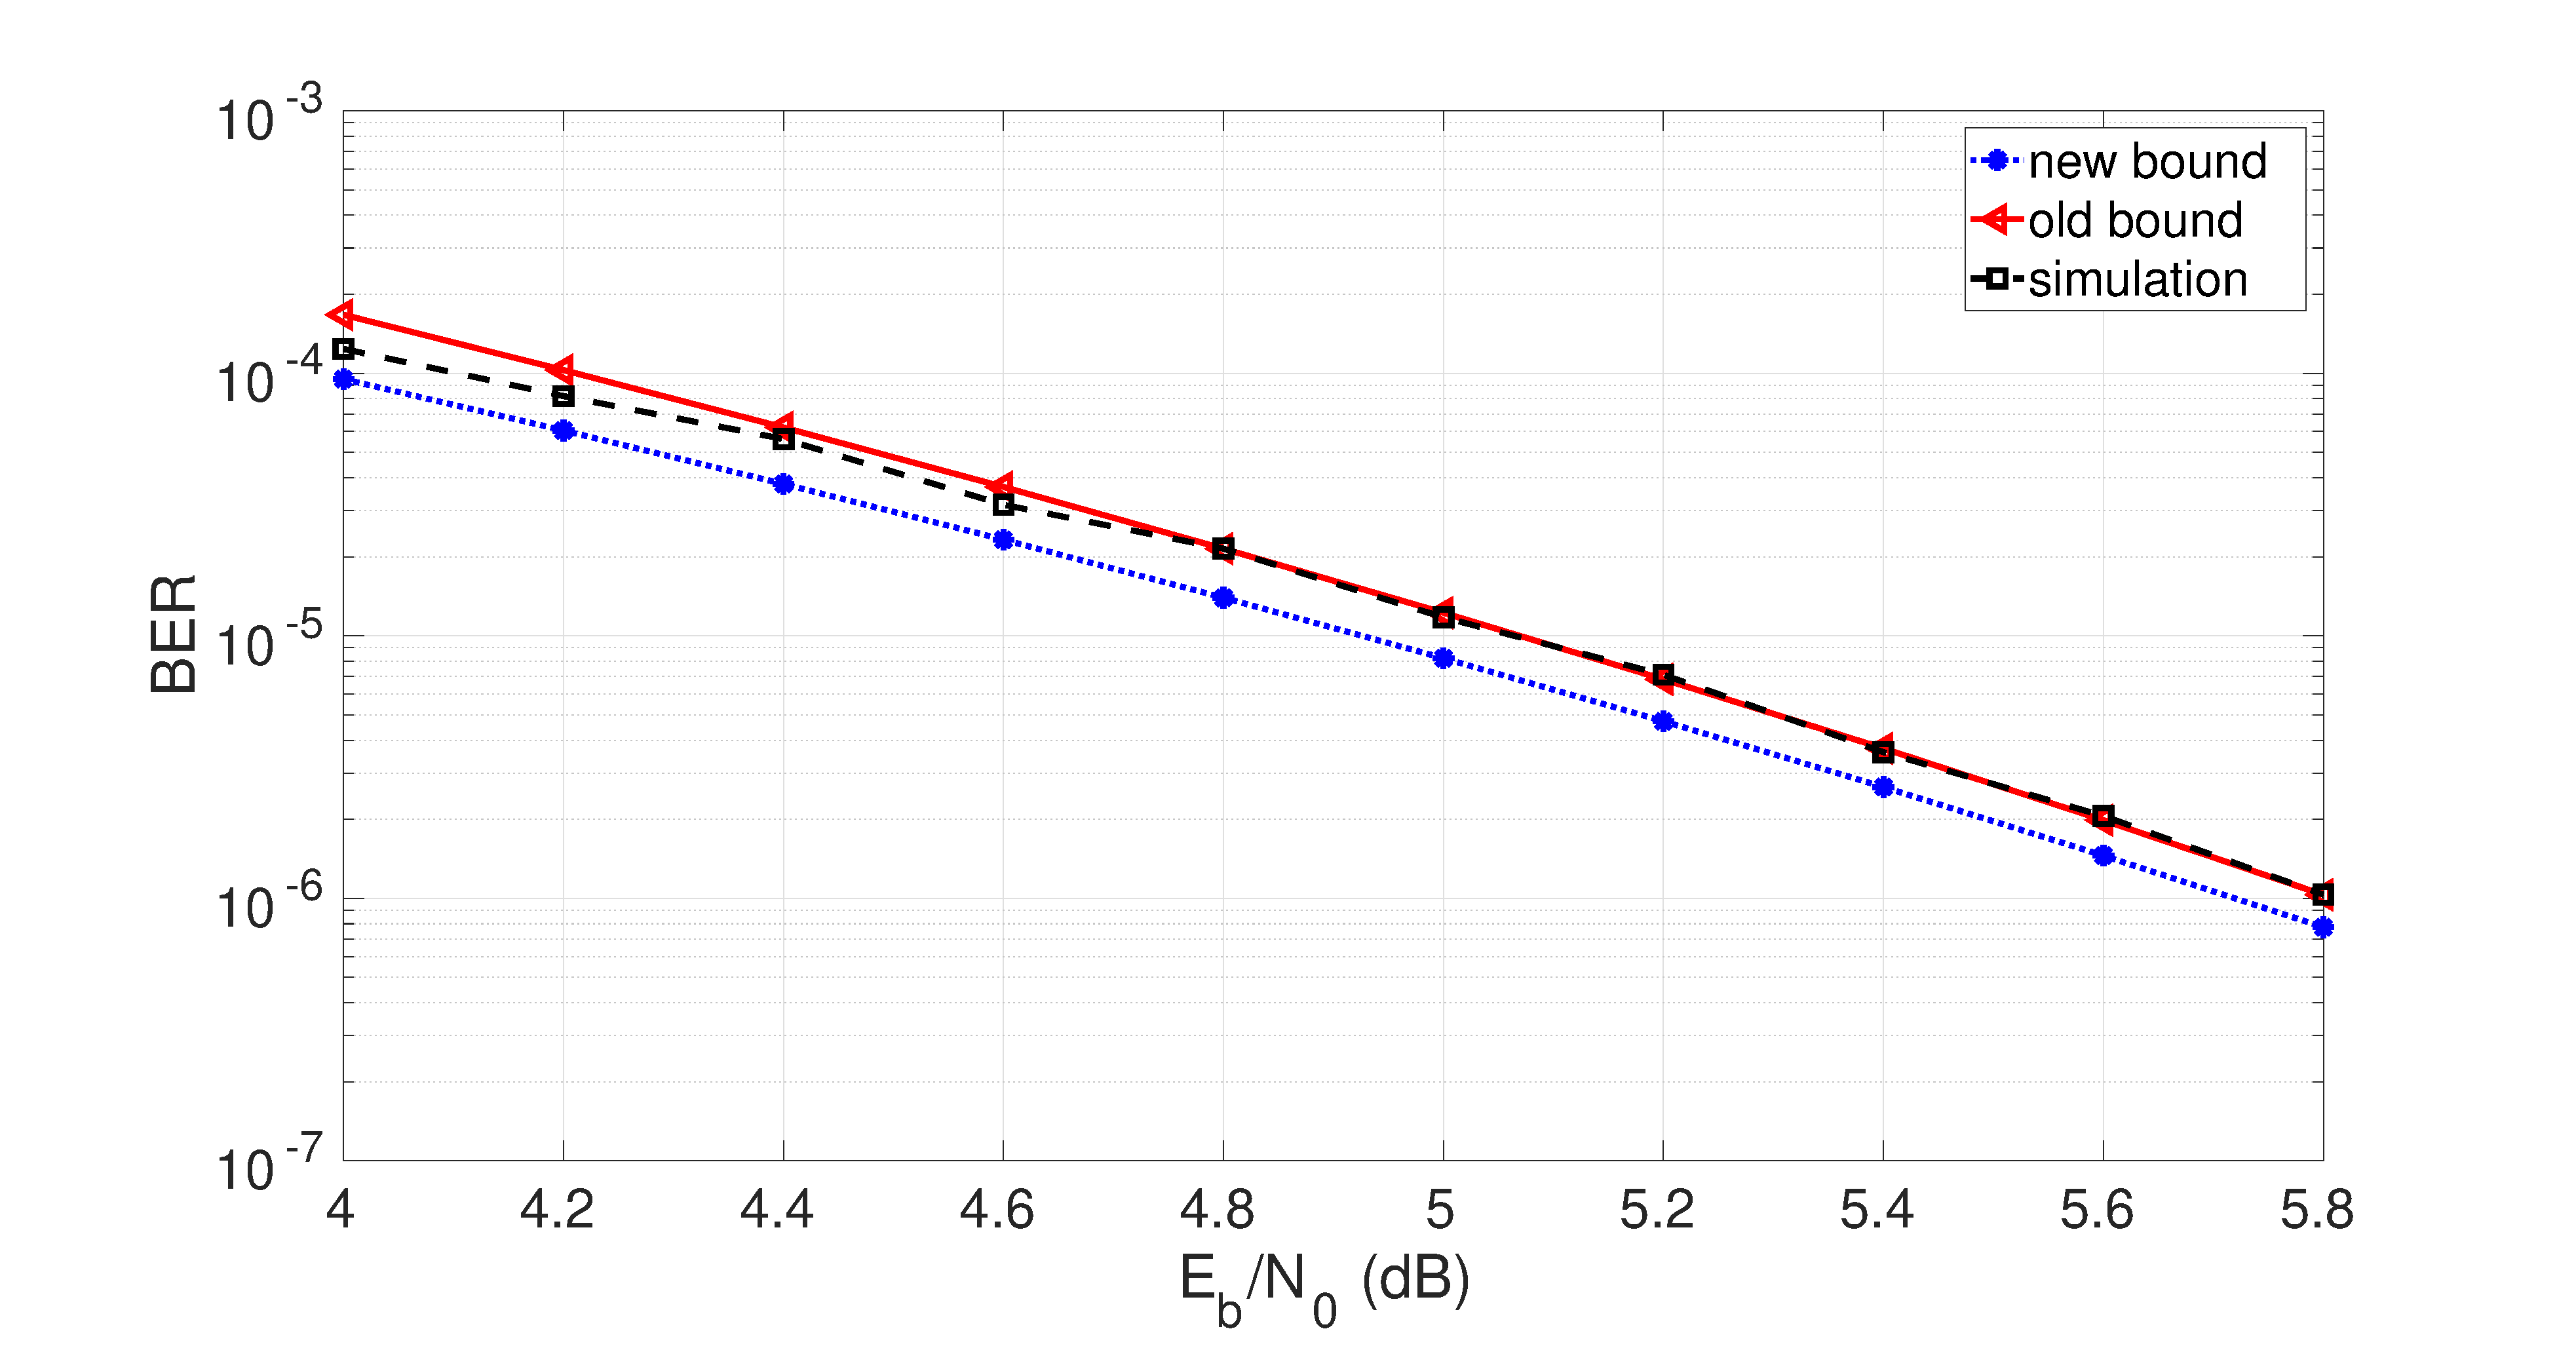
\includegraphics[width=0.5\textwidth]{./Images/RSC_23_35_lower_weights.eps}
		\caption{Old Bound vs New Bound vs Simulation for 23/35 RSC Code}
		\label{simFig3}
		\end{figure}
%Fig. \ref{simFig3} shows the simulation results for the $23/35$ RSC code as well as the lower bounds obtained using the transfer function as well as our novel method. The feedforward connection has the polynomial representation $1+x+x^4$, which is an irreducible polynomial. The low-weight codeword has parity check components of weight $2$ and weight $3$. However, since parity-check components yield high weight codewords, there are not included in our approximation of the lower bound, as can be observed from Table \ref{novelTab14}. The feedback connection has the polynomial representation $1+x^2+x^3+x^4$, which can be factorized into $2$ irreducible polynomials and there are no low-codewords with systematic components of weight $3$. In Fig. \ref{simFig3}, we observe that the old (transfer function) bounds and simulation results converge as the $E_b/N_0$ value increases. However, there is some difference between the new (novel method) bound and the old (transfer function) bound, even as $E_b/N_0$ increases. This suggests that the approximation used in our novel method is insufficient for this RSC code and considering  $w_H(h(x)),~w_H(b(x))=4$ might yield a more accurate bound.


%\begin{figure}[h!]
%\centering
%		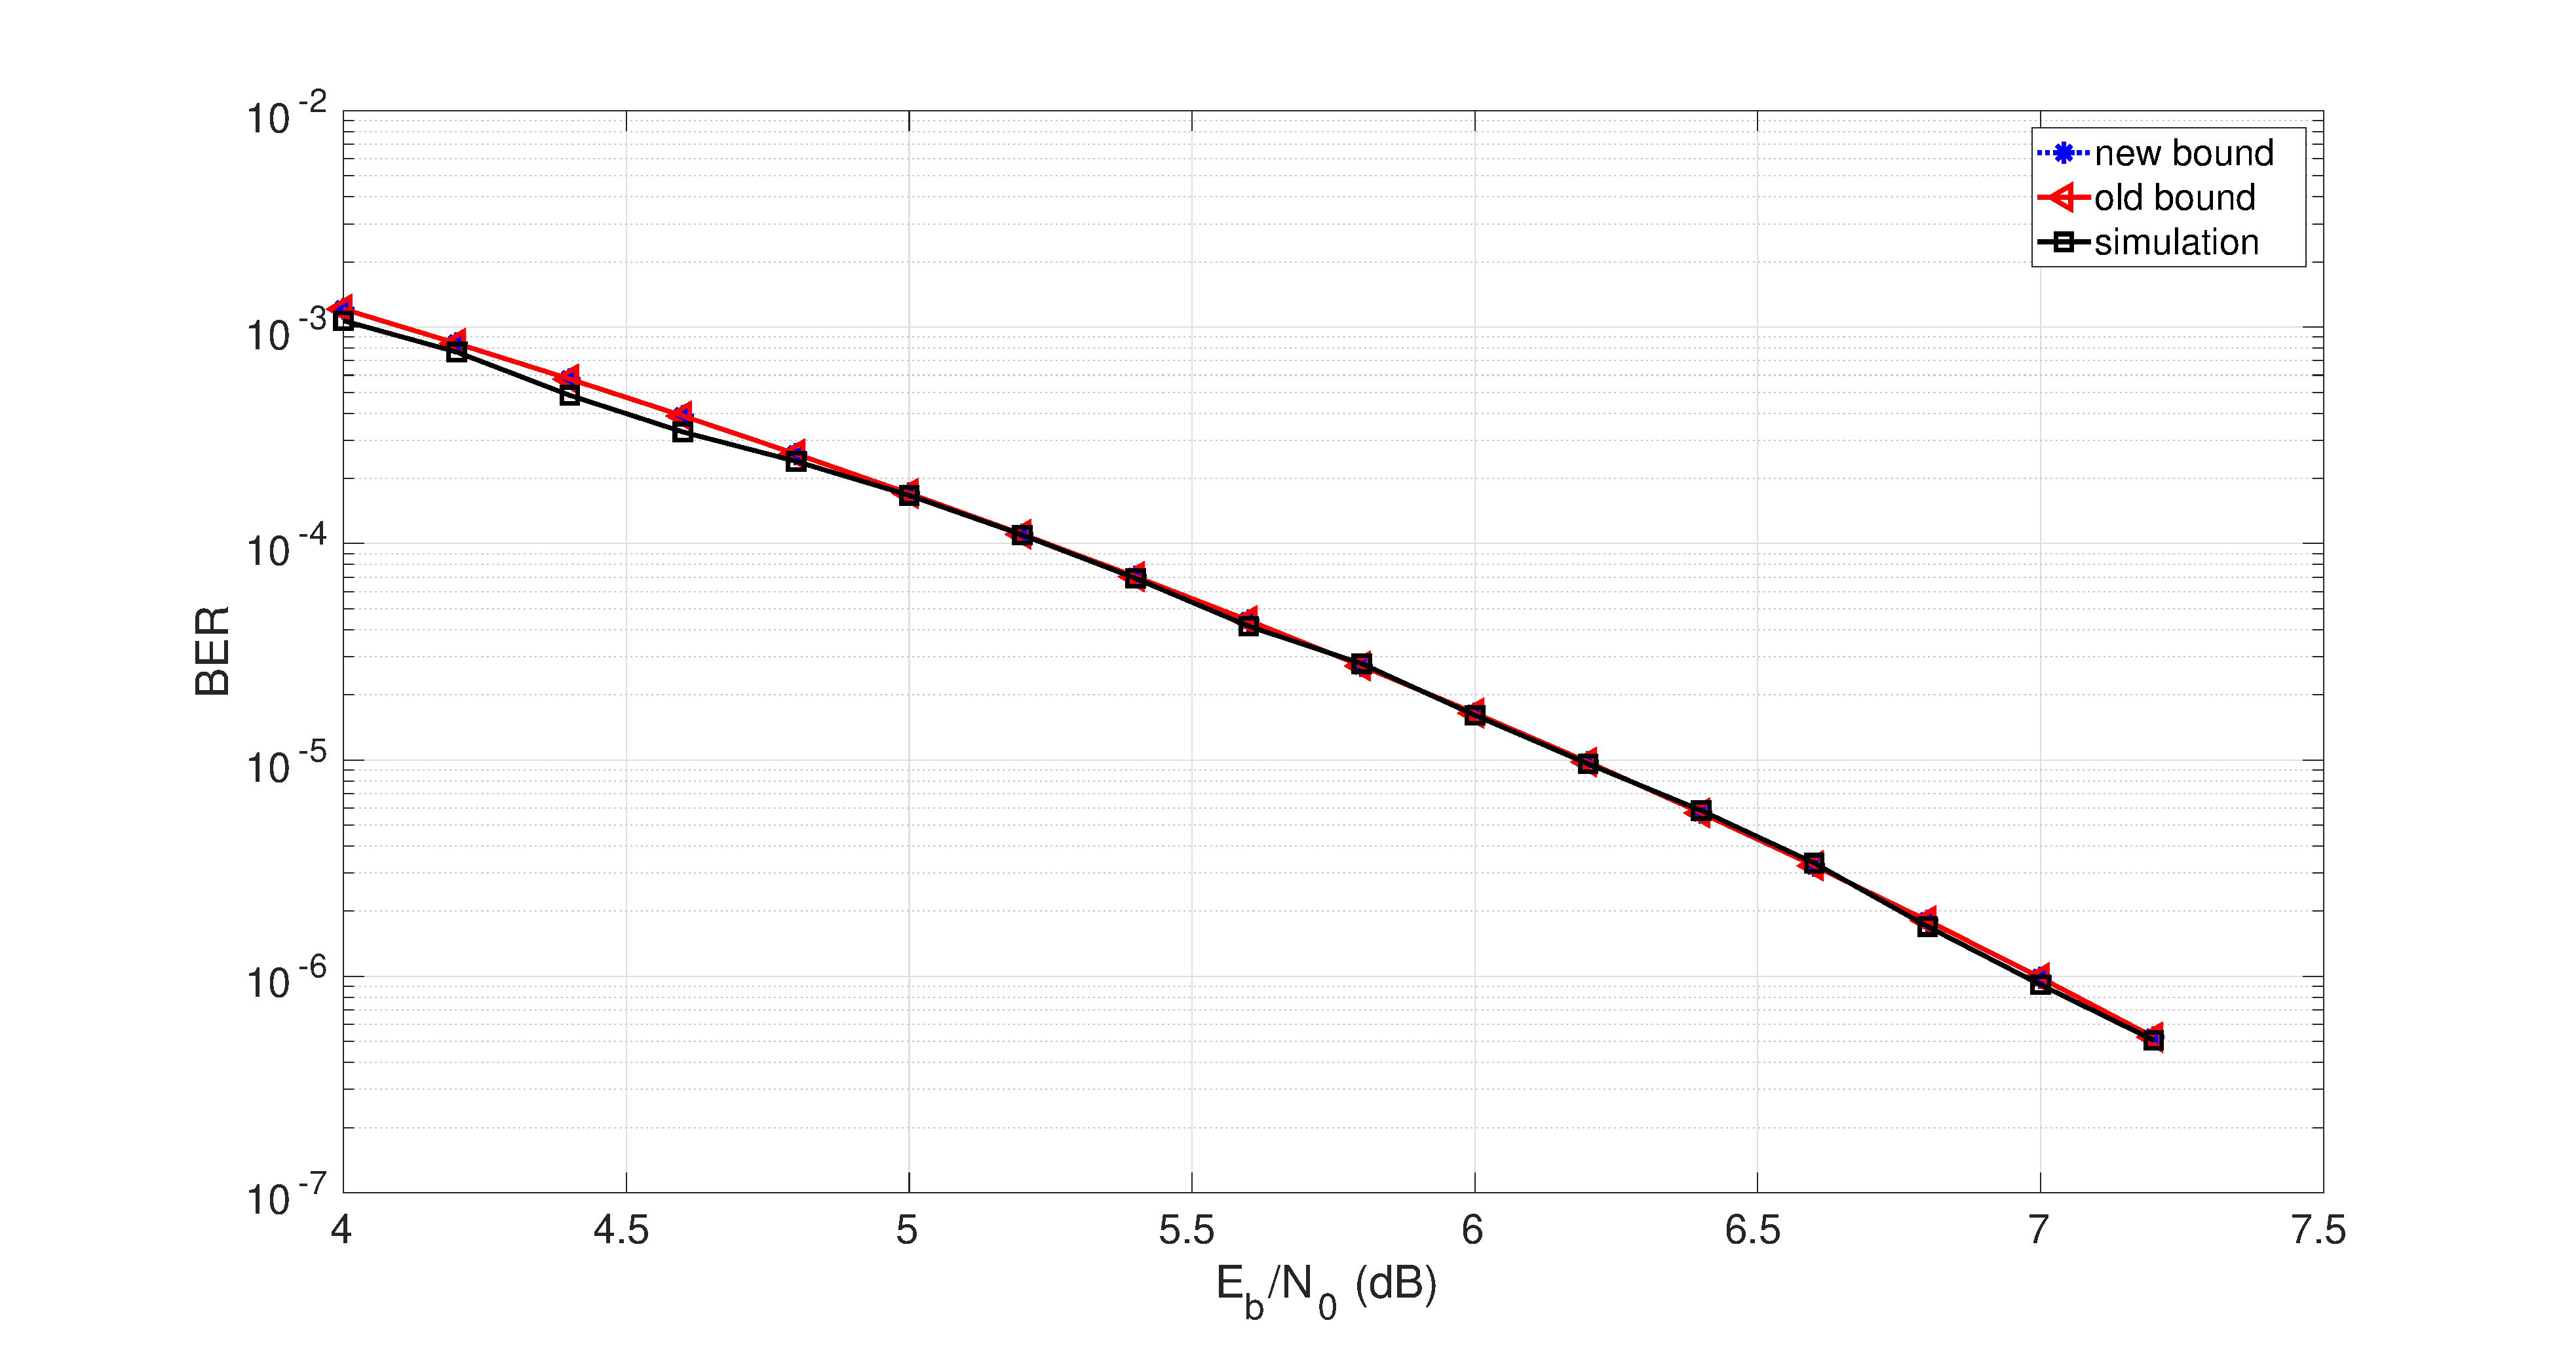
\includegraphics[width=0.8\textwidth]{./Images/RSC_5_7_higher_weights.eps}
%		\caption{Old Bound vs New Bound vs Simulation for 5/7 RSC Code, with higher weights }
%		\label{simFig4}
%		\end{figure}
		
		
%		\begin{figure}[h!]
%\centering
	%	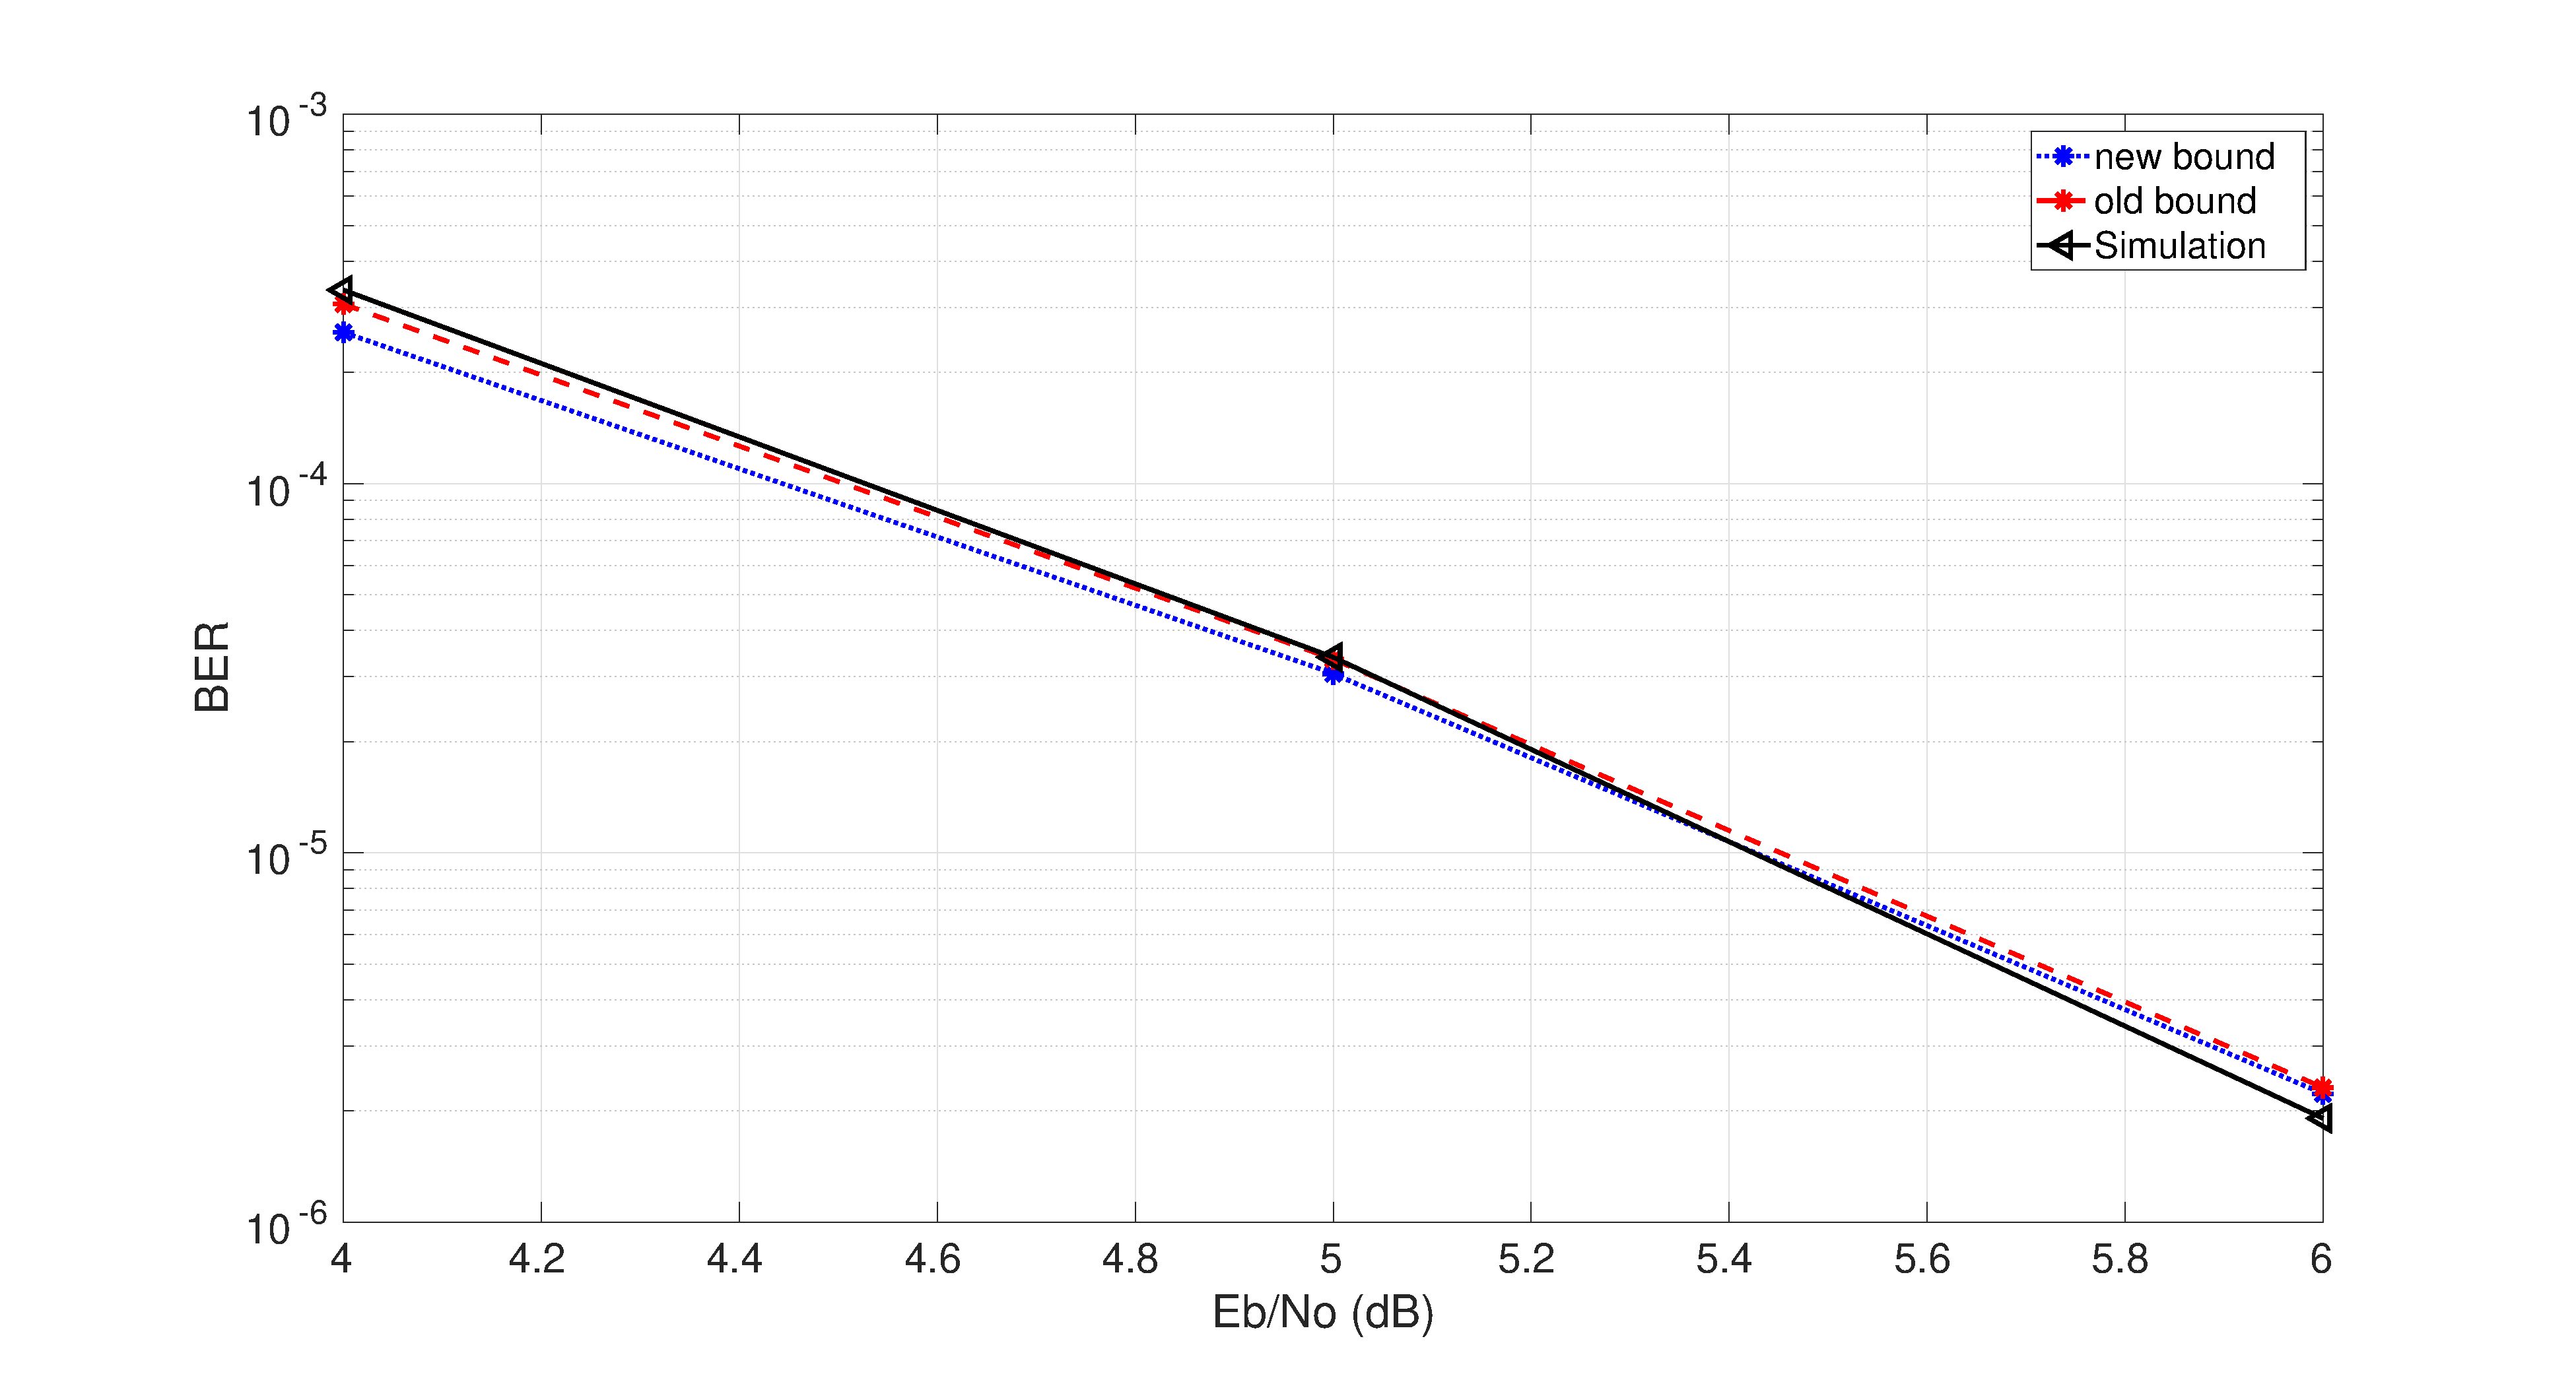
\includegraphics[width=0.5\textwidth]{./Images/RSC_37_21_v2.eps}
		%\caption{Old Bound vs New Bound vs Simulation for 37/21 RSC Code, with higher weights}
		%\label{simFig5}
		%\end{figure}



%\newpage
\section{Conclusion}
\label{sec6}
%In this paper,we presented a novel low-complexity method for determining the distance spectrum of any RSC code which has the added benefit of revealing the structure of the Return-To-Zero (RTZ) inputs that make up the distance spectrum as well as their corresponding parity-check sequences. 
%%%%%%%%%%%%%%%%%%%%%%%%%%%
%We then go a step further and present a method  for deriving a general polynomial representation for both RTZ inputs and parity-check sequences with a Hamming weight of up to $4$ for any RSC code.
 %%%%%%%%%%%%%%%%%%%%%%
 
% Combining these two methods, we list the partial distance spectrum for selected RSC codes up to a cut-off weight $d_{\text{max}}$ and compare simulation results to the bounds obtained via our novel method and the regular method.

%In this paper, we presented a method for listing input message which produce codewords with low-weight parity bit sequences for a for a given $(n,k)$ RSC code. Compared to the Transfer function method, it has low complexity and provides more information about distance spectrum of the RSCC. Using a specially configured finite state machine, we can obtain a partial distance spectrum which we use to calculate an upper bound for the RSCC.  


In this paper, we presented a method for listing the codeword component pattern distance spectrum for selected RSC codes up to a cut-off weight $d_{\text{max}}$ by focusing first on codewords with systematic components such that $2 \leq w_H(b(x)) \leq 3$, and then codewords with parity check components such that $2 \leq w_H(h(x)) \leq 3$. Compared to the transfer function method, it has low complexity and provides extra information with regard to the pattern of the low-weight codeword components $b(x)$ and $h(x)$, which makes it very useful for interleaver design. We compared the bounds obtained using our novel method with the bounds obtained via the transfer function as well as the simulation results for three RSC codes. Results show that whiles our method is sufficient for most RSC codes, considering codeword components with $w_H(h(x)), w_H(h(x)) =4$ in our approximation, might yield more accurate BER bounds.

\newpage
\begin{thebibliography}{99}
\bibitem{ref1}  C. Berrou, A. Glavieux and P. Thitimajshima, "Near Shannon limit error-correcting coding and decoding: Turbo-codes. 1," Proceedings of ICC '93 - IEEE International Conference on Communications, Geneva, Switzerland, 1993, pp. 1064-1070 vol.2, doi: 10.1109/ICC.1993.397441.
\bibitem{ref2} John G. Proakis, Masoud Salehi. ``Digital Communications'', 
Fifth Edition,Chapter 8, McGraw-Hill.
\bibitem{ref3} Todd K. Moon. ``Error Correcting Codes'',Chapter 12, John Wiley \& Sons.
\bibitem{ref4}Alain Glavieux, ``Channel Coding in Communication Networks: From Theory to Turbocodes'',\\ Chapter 3, John Wiley \& Son. 
\bibitem{ref5} Jing Sun and O. Y. Takeshita, "Interleavers for turbo codes using permutation polynomials over integer rings," in IEEE Transactions on Information Theory, vol. 51, no. 1, pp. 101-119, Jan. 2005, doi: 10.1109/TIT.2004.839478.
%\bibitem{ref6} C. Berrou, Y. Saouter, C. Douillard, S. Kerouedan and M. Jezequel, "Designing good permutations for turbo codes: towards a single model," 2004 IEEE International Conference on Communications (IEEE Cat. No.04CH37577), Paris, France, 2004, pp. 341-345, doi: 10.1109/ICC.2004.1312507.
\bibitem{ref7}R. Garzón-Bohórquez, C. Abdel Nour and C. Douillard, "Protograph-Based Interleavers for Punctured Turbo Codes," in IEEE Transactions on Communications, vol. 66, no. 5, pp. 1833-1844, May 2018, doi: 10.1109/TCOMM.2017.2783971.
\end{thebibliography}

\section{Submission of Papers for Review}

Papers in the form of a PDF file, formatted as described below, may be
submitted online at
\begin{center}
  \url{https://2021.ieee-isit.org/Papers.asp}
\end{center}
The deadline for registering the paper and uploading the manuscript is \textbf{January 27, 2021}.

A paper's primary content is restricted in length to \textbf{five pages} but
authors are allowed an optional sixth page only containing references.
The IEEEtran-conference style should be used as presented here.
Submissions should use a font size no smaller than 10 points and have reasonable margins on all the 4 sides of the text.

Each paper must be classified as ``eligible for student paper award''
or ``not eligible for student paper award''. \textbf{Do not include any text concerning the student paper award in the abstract or manuscript.}


\section{Submission of Accepted Papers}

Accepted papers will be published in full. A program booklet and a book of abstracts will also be
distributed at the Symposium to serve as a guide to the sessions.

The deadline for the submission of the final camera-ready paper will
be announced in due course.  Accepted papers not submitted by that
date will not appear in the ISIT proceedings and will not be included
in the technical program of the ISIT.


\section{Paper Format}

\subsection{Templates}

The paper (A4 or letter size, double-column format, not exceeding
5~pages) should be formatted as shown in this sample \LaTeX{} file
\cite{Laport:LaTeX, GMS:LaTeXComp, oetiker_latex, typesetmoser}.

The use of Microsoft Word instead of \LaTeX{} is strongly
discouraged. However, acceptable formatting may be achieved by using
the template that can be downloaded from the ISIT 2021 website:
\begin{center}
  \url{https://2021.ieee-isit.org/}
\end{center}

Users of other text processing systems should attempt to duplicate the
style of this example, in particular the sizes and type of font, as
closely as possible.


\subsection{Formatting}

The style of references, equations, figures, tables, etc., should be
the same as for the \emph{IEEE Transactions on Information
  Theory}. The source file of this template paper contains many more
instructions on how to format your paper. So, example code for
different numbers of authors, for figures and tables, and references
can be found (they are commented out).

%%%%%%
%% An example of a floating figure using the graphicx package.
%% Note that \label must occur AFTER (or within) \caption.
%% For figures, \caption should occur after the \includegraphics.
%%
% \begin{figure}[htbp]
%   \centering
%   \includegraphics[width=0.3\textwidth]{myfigure}
%   % where an .eps filename suffix will be assumed under latex,
%   % and a .pdf suffix will be assumed for pdflatex
%   \caption{Simulation results.}
%   \label{fig:sim}
% \end{figure}
%%%%%%

%%%%%%
%% An example of a double column floating figure using two subfigures.
%% (The subfigure.sty package must be loaded for this to work.)  The
%% subfigure \label commands are set within each subfigure command,
%% the \label for the overall figure must come after \caption.  
%% \hfil must be used as a separator to get equal spacing
%%
% \begin{figure*}[htbp]
%   \centerline{\subfigure[Case I]{\includegraphics[width=2.5in]{subfigcase1}
%       % where an .eps filename suffix will be assumed under latex,
%       % and a .pdf suffix will be assumed for pdflatex
%       \label{fig:first_case}}
%     \hfil
%     \subfigure[Case II]{\includegraphics[width=2.5in]{subfigcase2}
%       % where an .eps filename suffix will be assumed under latex,
%       % and a .pdf suffix will be assumed for pdflatex
%       \label{fig:second_case}}}
%   \caption{Simulation results.}
%   \label{fig:sim}
% \end{figure*}
%%%%%%

%%%%%%
%% An example of a floating table. 
%% Note that, for IEEE style tables, the \caption command should come
%% BEFORE the table. Table text will default to \footnotesize as IEEE
%% normally uses this smaller font for tables.  The \label must come
%% after \caption as always.
%%
% \begin{table}[htbp]
%   % increase table row spacing, adjust to taste
%   \renewcommand{\arraystretch}{1.3}
%   \caption{An Example of a Table}
%   \label{tab:table_example}
%   \centering
%   % Some packages, such as MDW tools, offer better commands for making tables
%   % than the plain LaTeX2e tabular which is used here.
%   \begin{tabular}{|c||c|}
%     \hline
%     One & Two\\
%     \hline
%     Three & Four\\
%     \hline
%   \end{tabular}
% \end{table}
%%%%%%


For instructions on how to typeset math, in particular for equation
arrays with broken equations, we refer to \cite{typesetmoser}.

Final papers should have no page numbers and no headers or footers (both will be added during the production of the proceedings).
The top and bottom margins should be at least 0.5 inches to leave room for page numbers.
The affiliation shown for authors should constitute a sufficient mailing
address for persons who wish to write for more details about the
paper.
All fonts should be embedded in the pdf file.

\subsection{PDF Requirements}

Only electronic submissions in form of a PDF file will be
accepted. The PDF file has to be PDF/A compliant. A common problem is
missing fonts. Make sure that all fonts are embedded. (In some cases,
printing a PDF to a PostScript file, and then creating a new PDF with
Acrobat Distiller, may do the trick.) More information (including
suitable Acrobat Distiller Settings) is available from the IEEE
website \cite{IEEE:pdfsettings, IEEE:AuthorToolbox}.


\section{Conclusion}

We conclude by pointing out that on the last page the columns need to
balanced. Instructions for that purpose are given in the source file.

Moreover, example code for an appendix (or appendices) can also be
found in the source file (they are commented out).

%%%%%%
%% Appendix:
%% If needed a single appendix is created by
%%
%\appendix
%%
%% If several appendices are needed, then the command
%%
% \appendices
%%
%% in combination with further \section-commands can be used.
%%%%%%

\section*{Acknowledgment}

We are indebted to Michael Shell for maintaining and improving
\texttt{IEEEtran.cls}. 


%%%%%%
%% To balance the columns at the last page of the paper use this
%% command:
%%
%\enlargethispage{-1.2cm} 
%%
%% If the balancing should occur in the middle of the references, use
%% the following trigger:
%%
\IEEEtriggeratref{4}
%%
%% which triggers a \newpage (i.e., new column) just before the given
%% reference number. Note that you need to adapt this if you modify
%% the paper.  The "triggered" command can be changed if desired:
%%
%\IEEEtriggercmd{\enlargethispage{-20cm}}
%%
%%%%%%


%%%%%%
%% References:
%% We recommend the usage of BibTeX:
%%
%\bibliographystyle{IEEEtran}
%\bibliography{definitions,bibliofile}
%%
%% where we here have assume the existence of the files
%% definitions.bib and bibliofile.bib.
%% BibTeX documentation can be obtained at:
%% http://www.ctan.org/tex-archive/biblio/bibtex/contrib/doc/
%%%%%%



%% Or you use manual references (pay attention to consistency and the
%% formatting style!):
\begin{thebibliography}{9}

\bibitem{Laport:LaTeX}
L.~Lamport,
  \emph{\LaTeX: A Document Preparation System,} 
  Addison-Wesley, Reading, Massachusetts, USA, 2nd~ed., 1994. 

\bibitem{GMS:LaTeXComp}
F.~Mittelbach, M,~Goossens, J.~Braams, D.~Carlisle, and
C.~Rowley, \emph{The {\LaTeX} Companion,} Addison-Wesley,
Reading, Massachusetts, USA, 2nd~ed., 2004.

\bibitem{oetiker_latex}
T.~Oetiker, H.~Partl, I.~Hyna, and E.~Schlegl, \emph{The Not So Short
  Introduction to {\LaTeX2e}}, version 5.06, Jun.~20, 2016. [Online].
  Available: \url{https://tobi.oetiker.ch/lshort/}

\bibitem{typesetmoser}
S.~M. Moser, \emph{How to Typeset Equations in {\LaTeX}}, version 4.6,
  Sep. 29, 2017. [Online]. Available:
  \url{http://moser-isi.ethz.ch/manuals.html#eqlatex}

\bibitem{IEEE:pdfsettings}
IEEE, \emph{Preparing Conference Content for the IEEE Xplore Digital
  Library.} [Online]. Available:
  \url{http://www.ieee.org/conferences_events/conferences/organizers/pubs/preparing_content.html}

\bibitem{IEEE:AuthorToolbox}
IEEE, \emph{Author Digital Toolbox.} [Online.] Available:
  \url{http://www.ieee.org/publications_standards/publications/authors/authors_journals.html}

\end{thebibliography}


\end{document}


%%%%%%
%% Some comments about useful packages
%% (extract from bare_conf.tex by Michael Shell)
%%

% *** MISC UTILITY PACKAGES ***
%
%\usepackage{ifpdf}
% Heiko Oberdiek's ifpdf.sty is very useful if you need conditional
% compilation based on whether the output is pdf or dvi.
% usage:
% \ifpdf
%   % pdf code
% \else
%   % dvi code
% \fi
% The latest version of ifpdf.sty can be obtained from:
% http://www.ctan.org/pkg/ifpdf
% Also, note that IEEEtran.cls V1.7 and later provides a builtin
% \ifCLASSINFOpdf conditional that works the same way.
% When switching from latex to pdflatex and vice-versa, the compiler may
% have to be run twice to clear warning/error messages.


% *** CITATION PACKAGES ***
%
%\usepackage{cite}
% cite.sty was written by Donald Arseneau
% V1.6 and later of IEEEtran pre-defines the format of the cite.sty package
% \cite{} output to follow that of the IEEE. Loading the cite package will
% result in citation numbers being automatically sorted and properly
% "compressed/ranged". e.g., [1], [9], [2], [7], [5], [6] without using
% cite.sty will become [1], [2], [5]--[7], [9] using cite.sty. cite.sty's
% \cite will automatically add leading space, if needed. Use cite.sty's
% noadjust option (cite.sty V3.8 and later) if you want to turn this off
% such as if a citation ever needs to be enclosed in parenthesis.
% cite.sty is already installed on most LaTeX systems. Be sure and use
% version 5.0 (2009-03-20) and later if using hyperref.sty.
% The latest version can be obtained at:
% http://www.ctan.org/pkg/cite
% The documentation is contained in the cite.sty file itself.


% *** GRAPHICS RELATED PACKAGES ***
%
\ifCLASSINFOpdf
  % \usepackage[pdftex]{graphicx}
  % declare the path(s) where your graphic files are
  % \graphicspath{{../pdf/}{../jpeg/}}
  % and their extensions so you won't have to specify these with
  % every instance of \includegraphics
  % \DeclareGraphicsExtensions{.pdf,.jpeg,.png}
\else
  % or other class option (dvipsone, dvipdf, if not using dvips). graphicx
  % will default to the driver specified in the system graphics.cfg if no
  % driver is specified.
  % \usepackage[dvips]{graphicx}
  % declare the path(s) where your graphic files are
  % \graphicspath{{../eps/}}
  % and their extensions so you won't have to specify these with
  % every instance of \includegraphics
  % \DeclareGraphicsExtensions{.eps}
\fi
% graphicx was written by David Carlisle and Sebastian Rahtz. It is
% required if you want graphics, photos, etc. graphicx.sty is already
% installed on most LaTeX systems. The latest version and documentation
% can be obtained at: 
% http://www.ctan.org/pkg/graphicx
% Another good source of documentation is "Using Imported Graphics in
% LaTeX2e" by Keith Reckdahl which can be found at:
% http://www.ctan.org/pkg/epslatex
%
% latex, and pdflatex in dvi mode, support graphics in encapsulated
% postscript (.eps) format. pdflatex in pdf mode supports graphics
% in .pdf, .jpeg, .png and .mps (metapost) formats. Users should ensure
% that all non-photo figures use a vector format (.eps, .pdf, .mps) and
% not a bitmapped formats (.jpeg, .png). The IEEE frowns on bitmapped formats
% which can result in "jaggedy"/blurry rendering of lines and letters as
% well as large increases in file sizes.
%
% You can find documentation about the pdfTeX application at:
% http://www.tug.org/applications/pdftex


% *** MATH PACKAGES ***
%
%\usepackage{amsmath}
% A popular package from the American Mathematical Society that provides
% many useful and powerful commands for dealing with mathematics.
%
% Note that the amsmath package sets \interdisplaylinepenalty to 10000
% thus preventing page breaks from occurring within multiline equations. Use:
%\interdisplaylinepenalty=2500
% after loading amsmath to restore such page breaks as IEEEtran.cls normally
% does. amsmath.sty is already installed on most LaTeX systems. The latest
% version and documentation can be obtained at:
% http://www.ctan.org/pkg/amsmath


% *** SPECIALIZED LIST PACKAGES ***
%
%\usepackage{algorithmic}
% algorithmic.sty was written by Peter Williams and Rogerio Brito.
% This package provides an algorithmic environment fo describing algorithms.
% You can use the algorithmic environment in-text or within a figure
% environment to provide for a floating algorithm. Do NOT use the algorithm
% floating environment provided by algorithm.sty (by the same authors) or
% algorithm2e.sty (by Christophe Fiorio) as the IEEE does not use dedicated
% algorithm float types and packages that provide these will not provide
% correct IEEE style captions. The latest version and documentation of
% algorithmic.sty can be obtained at:
% http://www.ctan.org/pkg/algorithms
% Also of interest may be the (relatively newer and more customizable)
% algorithmicx.sty package by Szasz Janos:
% http://www.ctan.org/pkg/algorithmicx


% *** ALIGNMENT PACKAGES ***
%
%\usepackage{array}
% Frank Mittelbach's and David Carlisle's array.sty patches and improves
% the standard LaTeX2e array and tabular environments to provide better
% appearance and additional user controls. As the default LaTeX2e table
% generation code is lacking to the point of almost being broken with
% respect to the quality of the end results, all users are strongly
% advised to use an enhanced (at the very least that provided by array.sty)
% set of table tools. array.sty is already installed on most systems. The
% latest version and documentation can be obtained at:
% http://www.ctan.org/pkg/array

% IEEEtran contains the IEEEeqnarray family of commands that can be used to
% generate multiline equations as well as matrices, tables, etc., of high
% quality.


% *** SUBFIGURE PACKAGES ***
%\ifCLASSOPTIONcompsoc
%  \usepackage[caption=false,font=normalsize,labelfont=sf,textfont=sf]{subfig}
%\else
%  \usepackage[caption=false,font=footnotesize]{subfig}
%\fi
% subfig.sty, written by Steven Douglas Cochran, is the modern replacement
% for subfigure.sty, the latter of which is no longer maintained and is
% incompatible with some LaTeX packages including fixltx2e. However,
% subfig.sty requires and automatically loads Axel Sommerfeldt's caption.sty
% which will override IEEEtran.cls' handling of captions and this will result
% in non-IEEE style figure/table captions. To prevent this problem, be sure
% and invoke subfig.sty's "caption=false" package option (available since
% subfig.sty version 1.3, 2005/06/28) as this is will preserve IEEEtran.cls
% handling of captions.
% Note that the Computer Society format requires a larger sans serif font
% than the serif footnote size font used in traditional IEEE formatting
% and thus the need to invoke different subfig.sty package options depending
% on whether compsoc mode has been enabled.
%
% The latest version and documentation of subfig.sty can be obtained at:
% http://www.ctan.org/pkg/subfig


% *** FLOAT PACKAGES ***
%
%\usepackage{fixltx2e}
% fixltx2e, the successor to the earlier fix2col.sty, was written by
% Frank Mittelbach and David Carlisle. This package corrects a few problems
% in the LaTeX2e kernel, the most notable of which is that in current
% LaTeX2e releases, the ordering of single and double column floats is not
% guaranteed to be preserved. Thus, an unpatched LaTeX2e can allow a
% single column figure to be placed prior to an earlier double column
% figure.
% Be aware that LaTeX2e kernels dated 2015 and later have fixltx2e.sty's
% corrections already built into the system in which case a warning will
% be issued if an attempt is made to load fixltx2e.sty as it is no longer
% needed.
% The latest version and documentation can be found at:
% http://www.ctan.org/pkg/fixltx2e


%\usepackage{stfloats}
% stfloats.sty was written by Sigitas Tolusis. This package gives LaTeX2e
% the ability to do double column floats at the bottom of the page as well
% as the top. (e.g., "\begin{figure*}[!b]" is not normally possible in
% LaTeX2e). It also provides a command:
%\fnbelowfloat
% to enable the placement of footnotes below bottom floats (the standard
% LaTeX2e kernel puts them above bottom floats). This is an invasive package
% which rewrites many portions of the LaTeX2e float routines. It may not work
% with other packages that modify the LaTeX2e float routines. The latest
% version and documentation can be obtained at:
% http://www.ctan.org/pkg/stfloats
% Do not use the stfloats baselinefloat ability as the IEEE does not allow
% \baselineskip to stretch. Authors submitting work to the IEEE should note
% that the IEEE rarely uses double column equations and that authors should try
% to avoid such use. Do not be tempted to use the cuted.sty or midfloat.sty
% packages (also by Sigitas Tolusis) as the IEEE does not format its papers in
% such ways.
% Do not attempt to use stfloats with fixltx2e as they are incompatible.
% Instead, use Morten Hogholm'a dblfloatfix which combines the features
% of both fixltx2e and stfloats:
%
% \usepackage{dblfloatfix}
% The latest version can be found at:
% http://www.ctan.org/pkg/dblfloatfix


% *** PDF and URL PACKAGES ***
%
%\usepackage{url}
% url.sty was written by Donald Arseneau. It provides better support for
% handling and breaking URLs. url.sty is already installed on most LaTeX
% systems. The latest version and documentation can be obtained at:
% http://www.ctan.org/pkg/url
% Basically, \url{my_url_here}.



% *** Do not adjust lengths that control margins, column widths, etc. ***
% *** Do not use packages that alter fonts (such as pslatex).         ***
%%%%%%


%%% Local Variables:
%%% mode: latex
%%% TeX-master: t
%%% End:
